%%
%%  thesis_latex_template_minimal.tex
%%
%%  A minimal working example using the LaTeX classfile umassdthesis.cls
%%  
%%  Grant O'Rielly
%%  grant.orielly@umassd.edu
%%
\documentclass[12pt,defaultstyle]{umassdthesis}

\usepackage[T1]{fontenc}
\usepackage[latin1]{inputenc}
\usepackage{graphicx}
%\usepackage[skip=0.5pt]{caption}
\usepackage{csquotes}
\usepackage{amsmath}
\usepackage{amsmath,mathtools}
\usepackage{amsfonts}
\usepackage{amssymb}
%\usepackage{gensymb} % for displaying degree celsius
\usepackage{siunitx}
\usepackage{tabularx}
\usepackage{makecell}
\usepackage{balance}
\usepackage{booktabs}
\usepackage{tabto}
\usepackage[none]{hyphenat}
\usepackage{float}
\usepackage{array}
\usepackage{verbatim}
\usepackage[noend]{algpseudocode}
\usepackage{algorithm}
\usepackage{subcaption}
\usepackage{csquotes}
\usepackage{enumitem}
\usepackage[none]{hyphenat}
\usepackage{acronym} 
\makeatletter
\def\BState{\State\hskip-\ALG@thistlm}
\makeatother
\usepackage{nomencl}
\makenomenclature
\frenchspacing
\usepackage{times} 
\usepackage{cases}
\def \b{\textbf}
\def \c{\mathcal}
\def \t{\text}
\def \T{\top}
\hyphenpenalty=2000
\tolerance=800
\newlist{abbrv}{itemize}{1}
\setlist[abbrv,1]{label=,labelwidth=1in,align=parleft,itemsep=0.1\baselineskip,leftmargin=!}
\usepackage{multirow,hhline,dcolumn} % useful commands for Tables
%\usepackage[toc]{appendix}
%\usepackage[pages]{appendix}

%%  user defined commands
\renewcommand{\arraystretch}{1}
\newcommand{\linefrac}[2]{\raisebox{.6ex}{#1}/\raisebox{-0.6ex}{#2}} 
\def\BibTeX{{\rm B\kern-.05em{\sc i\kern-.025em b}\kern-.08emT\kern-.1667em\lower.7ex\hbox{E}\kern-.125emX}}

%%  the entries below should be self-explanatory, some of these entries may
%%  safely be excluded from the thesis, other are required.  LaTeX will
%%  print a warning message if a required entry is not included.

\title{Cross-View Action Recognition via Joint Dictionary and Transfer Learning}

\author{Deepak}{Kumar}

\dept{College of}{Engineering}
\program{Data Science}
\college{College of}{Engineering}
\conferraldate{May}{2019}

%%  select the degree being earned
%%  \degree{FULL NAME}{ABBREVIATION}
%%
%\degree{Undergraduate}{Undergraduate}
%\degree{Honors}{Honors}
%\degree{Master of Arts}{M.A.}
%\degree{Master of Art Education}{M.A.Ed.}
%\degree{Master of Fine Arts}{M.F.A.}
\degree{Master of Science}{M.S.}

%%  PhD dissertations have extra details such as the program name
%%  and program label to allow for the EAS and BMBMT programs
%%
%%  \degree{Doctor of  Philosophy}{Ph.D.}
%%  \phdprogram{PROGRAM NAME}{LABEL}
%%
%\degree{Doctor of Philosophy}{Ph.D.}
%\phdprogram{Biomedical Engineering and Biotechnology}{BMEBT}
%\phdprogram{Computational Science}{EAS}
%\phdprogram{Computer Engineering}{ECE}


%%  advisors and readers have a professorial title, name,
%%  department and affiliation
%%  but NOT degrees earned (ie. do not write Dr. Smith)
%%
%%  eg. \advisor{PROFESSORIAL TITLE}{NAME}{DEPARTMENT}{AFFILIATION}
%%
\advisor{Assistant Professor}{Ming Shao}%
{Department of Computer and Information Science}{University of Massachusetts Dartmouth}

%%  co-advisors are allowed 
%%  sometime the co-advisor "replaces" a reader but othertimes
%%  there are also the full complement of readers.
%%  Undergraduate and Masters theses have two readers, while for
%%  Ph.D. dissertations, there are three readers.
%%  If the co-advisor replaces a reader simply leave one of the
%%  reader entries empty eg. \readerone{}{}{}{}
%%
%%  Also, if the same person has multiple roles 
%%  (eg. a reader and Department Chair) then their name should appear
%%  only once, with both roles acknowledged.
%% 
%%  The classfile can cope with all this potential ambiguity when 
%%  generating the signature page.
%% 
%\coadvisor{Associate Professor}{Fred A. Dagg}%
%{Physics}{University of Massachusetts Dartmouth}

\readerone{Assistant Professor}{David Koop}%
{Department of Computer and Information Science}{University of Massachusetts Dartmouth}

\readertwo{Assistant Professor}{Maoyuan Sun}%
{Department of Computer and Information Science}{University of Massachusetts Dartmouth}

%%  for readers with no academic affiliation
%%  the title and department entries are left empty and the affiliation entry
%%  includes the full address with LaTeX formatting mark-up.

%\readerthree{}{Luke Skywalker}%
%{}{Death Star Research Corporation\\Mos Eisley, Tatooine}


%%  the rest of the entries on the signature page have a
%%  professorial title and name (the affiliation will be UMASS DARTMOUTH)

\graddirector{David Koop}
\deptchair{Barry G. Dipper}
\collegedean{Jean VanderGheynst}
\gradstudies{Tesfay Meressi}
%%  this is for Honors (undergraduate) theses
%\honorsdirector{Catherine Gardner}

%%
%%  THE ABSTRACT
%%  ============
%%
%%  From the UMass Dartmouth Thesis Guide
%%  "Requirements for Theses and Dissertations" (Spring 2015) 
%%  
%%  5.1.4 Abstract
%%  --------------
%%  The thesis or dissertation must contain an abstract — a concise summary of
%%  the thesis or dissertation intended to inform a prospective reader about
%%  its content. It usually includes a brief description of the problem
%%  investigated, the procedures or methods used, the findings, and the
%%  conclusions. It may use one or a few paragraphs; however, it is very rare
%%  that an abstract should use more than two pages, and many use just one page. 
%%
\abstract[short]{%
  Human actions may be observed from multi-view, i.e., different cameras at the same time. Cross-view action recognition based on visual content is very challenging because the actions in different views may be internally related, but they look very different in the videos. With the help of improved dense trajectories (IDT), hand-crafted features satisfactory performance has been achieved on single-view, but these often fail for cross-view action recognition, due to non-discriminative features or feature space shift across the views.  In this study, we proposed a novel method for cross-view action recognition by getting discriminative features for each view and bringing them into a common subspace via a novel joint dictionary and transfer learning framework. The dictionary learning method aims to learn a structured dictionary shared by all classes, and the learned dictionary shares the latent representation of data through a group of linear mappings and learns the sparse discriminative coefficients for each view. In the meanwhile, the encoded discriminative features are projected to a common feature space across different views through transfer learning. The dictionary and transfer learning are alternatively optimized to ensure discriminative and transferable features for cross-view action recognition. The proposed method has been extensively evaluated on PKU-MMD dataset to validate the effectiveness of the proposed approach.
%%  the emply line before the closing brace is REQUIRED to ensure that 
%%  the formating of the abstract page is done correcty
%%  !!DO NOT REMOVE THIS LINE!!

}%
%%  done the abstract !!

%%
%%  THE ACKNOWLEDGEMENTS
%%  ====================
%%
%%  From the UMass Dartmouth Thesis Guide
%%  "Requirements for Theses and Dissertations" (Spring 2015) 
%%  
%%  5.1.5 Acknowledgments
%%  ---------------------
%%  Short statements of acknowledgment of indebtedness (e.g., thanks to one’s
%%  thesis or dissertation advisor, to other professors, to people who have
%%  given support) may appear on a separate page right after the abstract. An
%%  acknowledgments section is required if the author has received permission to
%%  use previously copyrighted material or is obliged to acknowledge grant
%%  sources. This section is present in most theses or dissertations and is used
%%  to express a very specific professional or personal indebtedness. For
%%  example, significant instances of collaboration with one or more others in
%%  one’s thesis or dissertation work would probably need acknowledgment in a
%%  Preface (see 5.1.8) or in this Acknowledgments section—for example, research
%%  undertaken together with another student or use of much material from some
%%  other investigator.
%%
%%  The acknowledgements should be written in a professional manner. When
%%  writing the acknowledgments, be sure that your use of “person” is
%%  consistent.  If you begin with references to yourself as “the author,”
%%  continue to use third person throughout. If you begin with first person
%%  (“I,” “me,” “my”), use first person consistently.  There are two accepted
%%  spellings of the word “acknowledgments” (the other is “acknowledgements”);
%%  be sure to spell this word consistently.
%%
\acknowledgements{%
  Foremost I would like to express my sincere appreciation and gratitude to my Thesis Advisor, Dr. Ming Shao, for the patient guidance, encouragement, motivation and advice he has provided. His guidance helped me in all the time of research and writing of this thesis. 
  
  I have been with Dr. Shao for the past two years, and he would meet with me regularly on a weekly basis even on summer and winter breaks. He was extremely quick in response to emails even during vacations. He had a confidence in me, and he pushed me through my good and bad times to give my best. He is the main reason that I am proceeding with my PhD at University of Massachusetts Dartmouth. It is my honor to work under his guidance.%\\
  
  %\noindent
  I would like to thank my Thesis Committee, Dr. David Koop and Dr. Maoyuan Sun for agreeing to be part of my thesis committee and their valuable feedback. %\\
  %\noindent
  
  At last but not least, I would like to thank my family, parents, siblings, cousins, my uncle and friends, for all kind of support that they provided me, and without them I would not be going for my PhD today.
%%  the emply line before the closing brace is REQUIRED to ensure that 
%%  the formating of the acknowledgments page is done correcty
%%  !!DO NOT REMOVE THIS LINE!!

}%
%%  done the acknowledgements !!


%%
%%  THE PREFACE (optional)
%%  ======================
%%
%%  From the UMass Dartmouth Thesis Guide
%%  "Requirements for Theses and Dissertations" (Spring 2015) 
%%  
%%  5.1.8 Preface (optional)
%%  ------------------------
%%  Most theses or dissertations will not have a Preface, which is called for
%%  only for unusual reasons, e.g., when the genesis of the work needs to be
%%  explained or when the author’s contribution to a multiple-authored work must
%%  be noted. If there is a preface, however, it would incorporate any
%%  acknowledgments instead of those appearing as a separate section.
%%  
%%  Preface sections are rarely used.  The first chapter (sometimes called
%%  “Introduction”) in the text section is the appropriate place for
%%  explanations of the context or the motivations that underlie the research,
%%  the research problem, the background of previous scholarship, notable
%%  contributions by other scholars, and so forth. Use a “Preface” section only
%%  for special purposes beyond such purposes as these; examples of such a
%%  special purpose are covered in sections 7.4 and 8.5.
%%  
%%
%%  7.4 Translations by the Author of Material Used
%%  ----------------------------------------------- 
%%  Material that you translate is still the intellectual property of the
%%  author. It must be documented fully (its original-language source cited
%%  properly and included in the bibliography). An appropriate note indicates by
%%  whom it has been translated, by you or someone else. If a thesis or
%%  dissertation will have extensive use of such material, this might be an
%%  occasion for an explanation in a Preface.  Usually, translators of published
%%  works will be indicated in the standard documentation of your notes and/or
%%  bibliography.
%% 
%%  8.5 Collaborative Work That Will Appear in a Thesis or Dissertation
%%  -------------------------------------------------------------------
%%  A thesis or dissertation must represent work done principally if not
%%  entirely by the author. When there are minor instances of research
%%  collaboration, an appropriate citation may be used. If extensive, however,
%%  the committee must approve it in detail and an explanation in a Preface
%%  section is called for (see sections 5.1.8).
%% 
%%  
%%  The preface should be written in a professional manner. When writing the
%%  acknowledgments, be sure that your use of “person” is consistent.  If you
%%  begin with references to yourself as “the author,” continue to use third
%%  person throughout. If you begin with first person (“I,” “me,” “my”), use
%%  first person consistently.  
%%
%\preface{%
%  The text of the preface goes here.
%%%  the emply line before the closing brace is REQUIRED to ensure that 
%%%  the formating of the preface page is done correcty
%%%  !!DO NOT REMOVE THIS LINE!!
%
%}%
%%%  done the preface !!


%%
%%  THE EPIGRAPH (optional)
%%  =======================
%%
%%  Some authors include a quotation (epigraph) or illustration (frontispiece)
%%  as the last of their preliminary pages. Neither should be listed in the
%%  table of contents, although a frontispiece may be included in the list of
%%  illustrations. The source of an epigraph is indicated below the quotation
%%  but is not listed in the bibliography or references unless it is also
%%  cited in the text. A page number need not be shown, but the page is
%%  counted in the sequential page numbering.

%%  The default option is a epigraph (text).
%%  The two LaTeX commands below will produce the same output.
%%
%\epigraph{%
%    \centering{To all of the fluffy kitties \ldots} 
%%%  the emply line before the closing brace is REQUIRED to ensure that 
%%%  the formating of the preface page is done correcty
%%%  !!DO NOT REMOVE THIS LINE!!
%
%}%
%\epigraph[epigraph]{%
%    \centering{To all of the fluffy kitties \ldots}
%%%  the emply line before the closing brace is REQUIRED to ensure that 
%%%  the formating of the preface page is done correcty
%%%  !!DO NOT REMOVE THIS LINE!!
%
%}%


%%  To include an illustration, use the optional argument of 
%%  frontispiece and the image file name as the second argument
%%
%\epigraph[frontispiece]{einstein_bike}

%%%  done the epigraph !!


%%  need these if there are no Figure or Tables
%%  otherwise evil things happen to the Table of Contents
%\emptyLoF
%\emptyLoT

%%  uncomment to aviod generating prologue pages
%\SuspendPrologue

%%  All the prologue pages are done.  The thesis proper begins after here.

%%
%%  End of LaTeX preamble
%%  =========================================================================

\begin{document}%
%\addcontentsline{toc}{chapter}{Abbreviation}%\addcontentsline{toc}{chapter}{Abbreviations} \noindent
\chapter*{Abbreviations}
%\setcounter{chapter}{3}
%\renewcommand{\thechapter}{\Roman{chapter}}
%\chaptermark{List of Abbreviations}
%\pagenumbering{arabic} 
%\setcounter{page}{2}

\begin{acronym}
	\acro{IDT}[IDT]{Improved Dense Trajectories}
	\acro{PCA}[PCA]{Principle Component Analysis}
	\acro{HOF}[HOF]{Histogram of Optical Flow}
	\acro{HOG}[HOG]{Histogram of Oriented Gradient}
	\acro{MBH}[MBH]{Motion Boundary Histogram}
	\acro{SVM}[SVM]{Support Vector Machine}
	\acro{TCA}[TCA]{Transfer Component Analysis}
	\acro{JDA}[JDA]{Joint Distribution Adaptation}
	\acro{BDA}[BDA]{Balanced Distribution Adaptation}
	\acro{TJM}[TJM]{Transfer Joint Matching}
	\acro{GMM}[GMM]{Gaussian Mixture Model}
	\acro{FV}[FV]{Fisher Vector} 
	\acro{DL}[DL]{Dictionary Learning}
	\acro{SIFT}[SIFT]{Scale Invariant Feature Transform}
	\acro{SURF}[SURF]{Speeded-up robust features} 
	\acro{LRSDL}[LRSDL]{Fast Low-Rank Shared Dictionary Learning}
	\acro{FDDL}[FDDL]{Fisher Discrimination Dictionary Learning}
	\acro{CCA}[CCA]{Canonical Correlation Analysis}
	\acro{LBP}[LBP]{Local Binary Pattern}
	\acro{LTP}[LTP]{Local Ternary Pattern}
	\acro{TL}[TL]{Transfer Learning}
\end{acronym}

	
	
	%\pagestyle{plain}
	%\setcounter{secnumdepth}{3}
	%\pagenumbering{arabic}
	% Input chapters
	%%\addcontentsline{toc}{chapter}{Abbreviations} \noindent
\chapter*{Abbreviations}
%\setcounter{chapter}{3}
%\renewcommand{\thechapter}{\Roman{chapter}}
%\chaptermark{List of Abbreviations}
%\pagenumbering{arabic} 
%\setcounter{page}{2}

\begin{acronym}
	\acro{IDT}[IDT]{Improved Dense Trajectories}
	\acro{PCA}[PCA]{Principle Component Analysis}
	\acro{HOF}[HOF]{Histogram of Optical Flow}
	\acro{HOG}[HOG]{Histogram of Oriented Gradient}
	\acro{MBH}[MBH]{Motion Boundary Histogram}
	\acro{SVM}[SVM]{Support Vector Machine}
	\acro{TCA}[TCA]{Transfer Component Analysis}
	\acro{JDA}[JDA]{Joint Distribution Adaptation}
	\acro{BDA}[BDA]{Balanced Distribution Adaptation}
	\acro{TJM}[TJM]{Transfer Joint Matching}
	\acro{GMM}[GMM]{Gaussian Mixture Model}
	\acro{FV}[FV]{Fisher Vector} 
	\acro{DL}[DL]{Dictionary Learning}
	\acro{SIFT}[SIFT]{Scale Invariant Feature Transform}
	\acro{SURF}[SURF]{Speeded-up robust features} 
	\acro{LRSDL}[LRSDL]{Fast Low-Rank Shared Dictionary Learning}
	\acro{FDDL}[FDDL]{Fisher Discrimination Dictionary Learning}
	\acro{CCA}[CCA]{Canonical Correlation Analysis}
	\acro{LBP}[LBP]{Local Binary Pattern}
	\acro{LTP}[LTP]{Local Ternary Pattern}
	\acro{TL}[TL]{Transfer Learning}
\end{acronym}

	\addcontentsline{toc}{chapter}{Abbreviation}%\addcontentsline{toc}{chapter}{Abbreviations} \noindent
\chapter*{Abbreviations}
%\setcounter{chapter}{3}
%\renewcommand{\thechapter}{\Roman{chapter}}
%\chaptermark{List of Abbreviations}
%\pagenumbering{arabic} 
%\setcounter{page}{2}

\begin{acronym}
	\acro{IDT}[IDT]{Improved Dense Trajectories}
	\acro{PCA}[PCA]{Principle Component Analysis}
	\acro{HOF}[HOF]{Histogram of Optical Flow}
	\acro{HOG}[HOG]{Histogram of Oriented Gradient}
	\acro{MBH}[MBH]{Motion Boundary Histogram}
	\acro{SVM}[SVM]{Support Vector Machine}
	\acro{TCA}[TCA]{Transfer Component Analysis}
	\acro{JDA}[JDA]{Joint Distribution Adaptation}
	\acro{BDA}[BDA]{Balanced Distribution Adaptation}
	\acro{TJM}[TJM]{Transfer Joint Matching}
	\acro{GMM}[GMM]{Gaussian Mixture Model}
	\acro{FV}[FV]{Fisher Vector} 
	\acro{DL}[DL]{Dictionary Learning}
	\acro{SIFT}[SIFT]{Scale Invariant Feature Transform}
	\acro{SURF}[SURF]{Speeded-up robust features} 
	\acro{LRSDL}[LRSDL]{Fast Low-Rank Shared Dictionary Learning}
	\acro{FDDL}[FDDL]{Fisher Discrimination Dictionary Learning}
	\acro{CCA}[CCA]{Canonical Correlation Analysis}
	\acro{LBP}[LBP]{Local Binary Pattern}
	\acro{LTP}[LTP]{Local Ternary Pattern}
	\acro{TL}[TL]{Transfer Learning}
\end{acronym}

	\chapter{Introduction}
\label{intro}

\pagenumbering{arabic} 


Action recognition is an active research field, which has received considerable attention in computer vision in the past decade. The major goal of action recognition is to automatically understand different types of actions to reduce human workload. The ever-growing interest in recognizing human actions is in part due to the wide range of applications, including, but not limited to the following:

\noindent
\textbf{Intelligent Visual Surveillance.} There are number of cameras deployed for security surveillance to monitor criminal or suspicious activities, but these require constant human monitoring. To minimize the human workload, intelligent visual surveillance systems can be used to automatically detect and recognize suspicious activities and can generate alerts to security personnel~\cite{xiang2008video} in order to prevent any dangerous situations.
\begin{figure}[!ht]
\begin{center}
	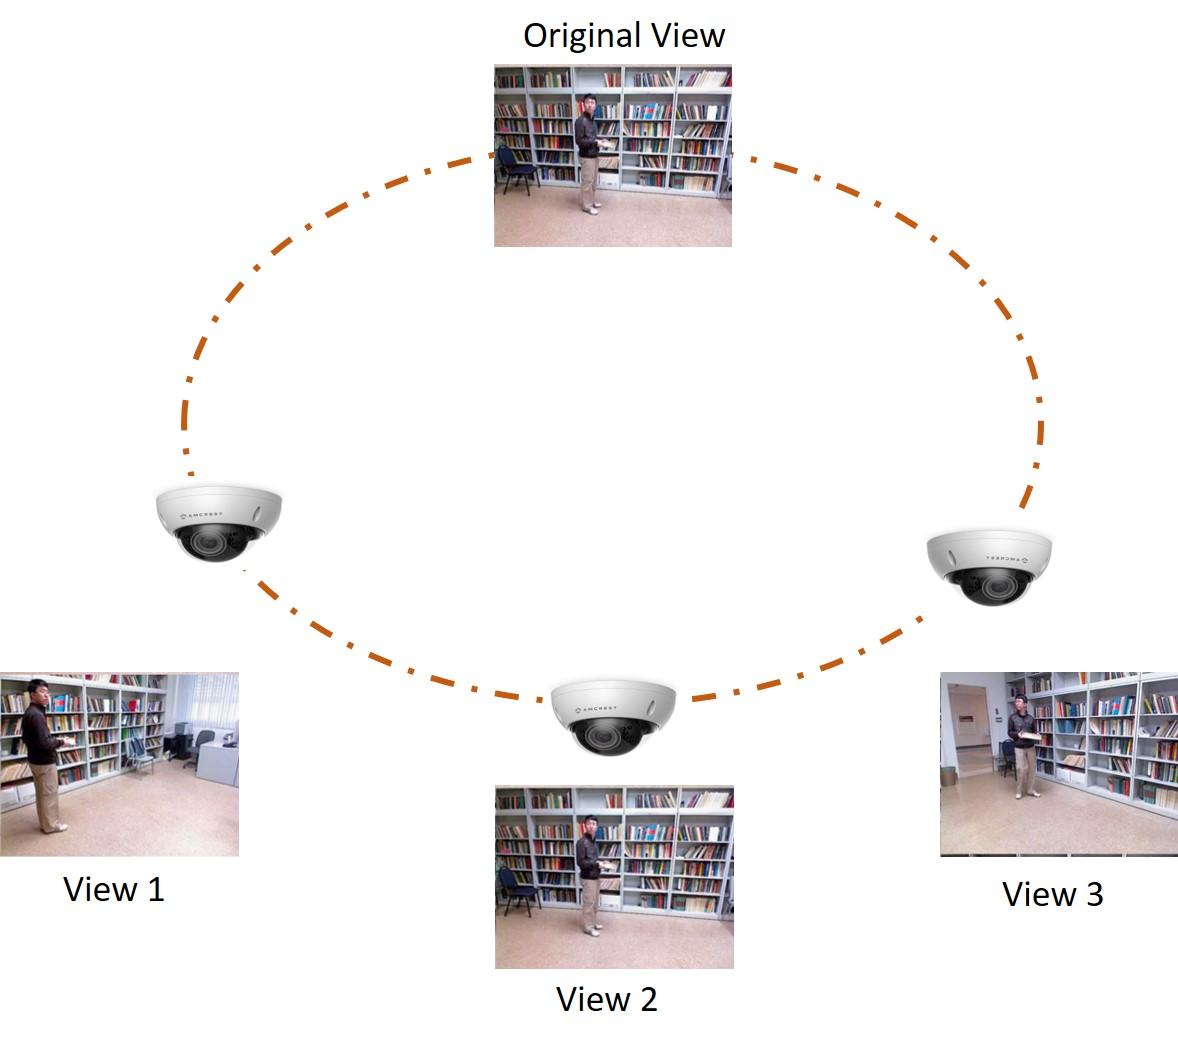
\includegraphics[width=4.5in,height=4in]{figures/motivationfigure.jpg}
	\linebreak
	\captionof{figure}{Illustration of cross-view action recognition in surveillance system.}
	\label{fig1:MEHTODILL}
\end{center}
\end{figure}

\noindent
\textbf{Ambient Assisted Living.} Ambient assisted living systems are used in health care \cite{MUBASHIR2013144} to automatically monitor and analyze patient activities, and also daily life activities especially for elderly people such as falling down, having a stroke or respiration issue, etc.

\noindent
\textbf{Human-computer Interaction.} Human gestures can be used to operate different tasks in the computer such as changing presentation slides using hand gestures instead of using traditional methods such as keyboard and mouse~\cite{799904}.

\noindent
\textbf{Entertainment.} The modern era of gaming uses the human body as a controller instead of using gaming controllers. These systems can be used to track a player's activity during his or her interaction with the gaming environment~\cite{VALLIM20136258}.
%\\
%There are number of action recognition studies have been carried out but it still remains very challenging task, mainly because there is usually large amount of viewpoint variations, different illumination conditions, occlusion, variance in human appearance, shape, clothes, cluttered backgrounds, stationary and moving cameras.\\
%\noindent\textcolor{blue}{

Considerable work is done for single view action recognition when videos are captured from a fixed view using one camera~\cite{sharma2013expanded,liang2013learning,wu2014multi,benmokhtar2014robust,papadopoulos2014real}. However, from the above-mentioned applications, there can be multiple cameras to capture a single action from different viewpoints or angles to get enriched information for action description as shown in Figure~\ref{fig1:MEHTODILL}, where single object actions are captured by three different cameras fixed at three different angles. Most of the proposed approaches  for single view or multi-view action recognition consist of feature engineering which includes different feature extraction~\cite{Efros:2003:RAD:946247.946720,4270156,5459184,wang2013action,1238378}, dictionary learning~\cite{8082519,4483511,zheng2016cross}, and deep learning~\cite{deng2014deep} methods.
However, it is still challenging to recognize action from different view points because the same action looks quite different across views. There are a couple of methods proposed for multi-view or cross-view action recognition, but multiple challenges still remain which need to be addressed~\cite{ji2010advances,holte2011human}.
%\\

The first key step for action recognition is to extract features from video frames. Feature extraction can be understood as a process of retrieving values at the pixel level which is informative and non-redundant. These values give us points of interest which on their own do not contribute to the action itself but extract most relevant points from the raw data. There are challenges in feature extraction, like cluttered images where it is hard to differentiate objects from one another, similarity in colors between objects, camera motion which can bring noise in the images and create blurred frames, large amount of viewpoint variations, different illumination conditions, occlusion, variance in human appearance, shapes, clothes, etc. Another major challenge in this process is selecting a suitable framework that can represent the extracted features accurately and also take into consideration the changes in the spatial and temporal information.
Many feature representation methods are proposed for action recognition in video sequences, such as optical flow patterns~\cite{Efros:2003:RAD:946247.946720,1315182}, shape feature~\cite{4270156,5459184,1211340,4587527}, space-time pattern templates~\cite{1467373,1544882} dense trajectories~\cite{wang2013dense}, improved dense trajectories~\cite{wang2013action}, and spatio-temporal interest points~\cite{1238378}. Although these handcrafted low-level feature methods are powerful to recognize actions in similar view or in controlled scenarios, the performance degrades with viewpoint changes. One reason is appearance difference when observed from different angles, due to this along with view change, the low-level features become less discriminative. One possible solution is brutal-force approach that trains a separate classifier for each view, but it becomes intractable as the number of action categories and views increase. In addition, it is computationally expensive or infeasible to train a separate classifier to address the action under novel views. Another approach is to build view invariant~\cite{10.1007/978-3-540-88688-4_22,6939719,zheng2016cross,zheng2013learning, 7045574, 7907301,6958807} representation for action recognition. 

Although these low-level features achieved great success, designing the effective discriminative features requires the new domain knowledge and these hand-crafted features cannot simply be adapted to new conditions. Learning feature from data itself is considered a plausible way to overcome these limitations and successful examples are dictionary learning and deep learning.
%\\
The idea of deep learning is to discover multiple levels of representation~\cite{deng2014deep}, that deeply learned features will represent the abstract semantics of data. It is expected from deep learning models, that these will provide features which will be more invariant to intra-class variability. The issue with deep learning is that it requires the large amount of labeled data to train a model, and in some cases, it is impossible or not practical. Sometimes pre-trained models are used for feature extraction and then weights of these pre-trained models are fine-tuned. However, the effectiveness of the \enquote{transferred} features becomes worse when source and target become less similar.
 
 %\\
 %\noindent
 In contrast, dictionary learning (DL) methods have demonstrated great success in image classification tasks on both small and large intra-class variation datasets~\cite{8082519}. The last few years have witnessed the fast development of DL methods under sparse representation theory, i.e., signals can be well-approximated by the linear combination of few columns of some basis or dictionary~\cite{4483511}. The dictionary that faithfully and discriminatively encodes signals plays an important role in the success of sparse representation. Conventional dictionary learning performs well for different classification and recognition tasks, but the performance deteriorates for cross-view action recognition. The primary reason is discriminative features for each view are not in common feature subspace. Notably, there are view-shared sparse representation based approaches proposed~\cite{zheng2013learning,zheng2016cross}. In those approaches, they assumed that different views contribute equally in shared features, and they ignored view-private features, however, it is not always valid.  
 
 Another approach is to incorporate transfer learning to bring the source and target in the common subspace. Transfer learning aims to improve the learning of target predictive function using the source knowledge.
Transfer learning tries to bring the distribution of source and target domain in the common subspace by learning knowledge from one or more source domains and transfer that to target domain in order to improve the performance~\cite{Weiss2016}.
The main purpose is to find the common representative for the similar objects which look different when they are in different views.

% Transfer learning definition
 Transfer learning can be performed in supervised, semi-supervised and unsupervised ways. In supervised learning~\cite{daume2009frustratingly, chattopadhyay2012multisource} the source and target both contain labeled data, in semi-supervised~\cite{chattopadhyay2012multisource,blitzer2006domain1} source domain has labeled data, while target domain has limited or no labeled data, and in unsupervised~\cite{cook2013transfer} there is no labeled data for both source and target domains. In brief, transfer learning may help to improve the performance for cross-view action recognition, but with performance being compromised, because source and target may not be discriminative in common space.   

\section{Motivation}
Considerable feature representation methods have been proposed for action recognition in videos, but these are only powerful for same view action recognition. In that sense, the performance degrades when the same action is performed from a different view. Recent learning approaches have cast a light on such issues. First, transfer learning or domain adaptation methods have shown good results for such scenarios, but this approach is largely limited by discriminant ability because the features brought up in the common subspace neither promotes the underlying sparse structure of data, nor preserve the best features. Second, shared dictionary learned for cross-view action recognition provides sparse representation, but it may ignore view private features. In some cases, e.g., when actions are performed from unseen views which are not part of the shared dictionary, the performance will degrade significantly.

Motivated by the above analysis and the limitation of transfer learning and dictionary learning for cross-view action recognition when these methods are incorporated separately, we proposed a novel approach called \textbf{Joint Dictionary and Transfer Learning (JDTL)} that helps to improve the performance of cross-view action recognition, where dictionary learning pursues the discriminative and robust representation for each view and transfer learning aims to bring those discriminative features of each view in the common subspace.
\newpage
\section{Contribution}
The main technical contributions of this work are:
\begin{itemize}
\item We pursue discriminant dictionary learning in each view with $D^{(v)}$ as the $v$-th view dictionary and  $X^{(v)}$ as the coding and we learned view independent dictionaries $D^{(v)} = [D_1^{(v)},D_2^{(v)},\cdots,D_C^{(v)}]$ to extract discriminative features for $C$ different actions. A common feature space will be optimized through transfer learning across different views in a joint learning framework with dictionary learning.
\item An iterative optimization is developed to approach our learning problems where the transfer learning projection matrix $P$, dictionary $D$ and coefficients $X$ are learned simultaneously. In each iteration, the coefficients $X$ are updated by fixing $P$ and $D$, dictionary $D$ is refined by fixing the $P$ and $X$, and $P$ is learned by fixing $D$ and $X$. The learning process will terminate until the objective converges.
\item To evaluate the proposed method, extended experiments have been performed on PKU-MMD dataset~\cite{liu2017pku}, a benchmark multi-view action recognition dataset. Experimental results demonstrate that our proposed method has achieved promising results for cross-view action recognition.
\end{itemize}

% 1). We introduce $D^{(v)}$ as the v-th view dictionary and  $X^{(v)}$ as the v-th coding and we learned view independent dictionaries $D^{(v)} = [D_1^{(v)},D_2^{(v)},\cdots,D_C^{(v)}]$ to extract discriminative features for $C$ actions. 
% %The main contribution of our work is given in two-folds. First, the success of dictionary learning inspires us to learn view-independent dictionaries for each view. 
% 2)These discriminative features are projected in common subspace through transfer learning across different views.}\\
% \noindent
% Our proposed method is an iterative process where the transfer learning projection matrix $P$, dictionary $D$ and coefficients $X$ are learned simultaneously. In each iteration, the coefficients $X$ are updated by fixing $P$ and $D$, and refines the dictionary $D$ by fixing the $P$ and $X$, while $P$ is learned by fixing $D$ and $X$. The aim is to get optimized projection matrix $P$, dictionary $D$ and coefficients $X$. \\
% \noindent
% To evaluate the proposed method, an extended experimentation is performed on PKU-MMD dataset~\cite{liu2017pku}, a benchmark multi-view action recognition dataset.\ Experimental results demonstrate that our proposed method has achieved significant results for cross-view action recognition. 
\section{Outline}
This thesis consists of 6 chapters including the introduction. Chapter 2 reviews the recent work. Chapter 3 presents the proposed joint dictionary and transfer learning method. Dataset preprocessing and experimental setup are described in Chapter 4. Experimental results and evaluation of our method are discussed in Chapter 5 and we present future work and draw the conclusion in Chapter 6.  







	\chapter{Literature Review}
\label{LR}
%\pagenumbering{arabic} 

A comprehensive review of the different types of visual handcrafted features for action recognition will be discussed in this chapter. What follows is recent learning techniques including dictionary and transfer learning.

\section{Hand-Crafted Features}
In handcrafted method, local features are extracted using space-time interest points~\cite{Laptev2005}, cuboids~\cite{6126543}, dense trajectories~\cite{HengWang:2011:ARD:2191740.2192078} and improved dense trajectories~\cite{wang2013action}. Local features are calculated with the help of detectors and descriptors, which are introduced below.
\subsection{Feature Detection}
A simple definition for feature detection is to detect locations of interest points and to check if there are features available at those locations. A few commonly used methods are described below. %\\

\noindent
\textbf{Harris3D Detector.~}
Harris3D detector detects local structures in space-time, where there is significant local variation in the image space and time. This means that the Harris 3D detector can detect similar regions in images by using affine transformations which has different illuminations~\cite{Laptev2005}. This is particularly useful when the same image is taken from different angles and similar regions need to be identified.%\\

\noindent
\textbf{Cuboid Detector.~}
The main task was to detect the spatio-temporal interest points. The main difference in this detector is that it makes use of two separate linear filters for both spatial and temporal dimensions instead of using a 3D filter~\cite{Dollar:2005:BRV:1259587.1259830}.%\\

\noindent
\textbf{Hessian Detector.~}
The hessian detector was proposed in~\cite{Willems2008}, and it is used for blob detection in images. It is an extension of the hessian saliency measure. The second-order Taylor expansion of the intensity surface is explored and especially the hessian matrix (containing the second order derivatives). 
The matrix determinant reaches a maximum in the image for blob-like structure~\cite{tuytelaars2008local12}. %\\

\begin{equation}
	 H = 
	\begin{bmatrix}
	I_{xx}(X, \sigma_D)&I_{xy}(X, \sigma_D)\\
	I_{xy}(X, \sigma_D)&I_{yy}(X, \sigma_D)\\
	\end{bmatrix}
	\label{eq:hassian}
\end{equation}
%\noindent
The 2$\times$2 matrix given in equation~\ref{eq:hassian} is the hessian matrix generated from the Taylor expansion of the image intensity function $I(X)$. where $I_{xx}$ is the second-order gaussian smoothed image derivatives which encodes the shape information and captures the local image structure. 
The filters based on the determinant and the trace of this matrix are particularly interesting. The latter is often referred as the Laplacian. The blob-like image structure is detected by calculating the local maxima of both measurements. The drawback of Laplacian filter is that signal changes in one direction while local maxima is found close to contours or straight edges.%\\

\noindent
\textbf{Dense Sampling.~}
In dense sampling, video blocks are extracted at regular positions and scales in space and time~\cite{6233178}. The data/video is sampled from five dimensions $x, y, t, \sigma,  \tau$.   Here $\sigma$  and $\tau$   represent the spatial and temporal scale.\ Dense sampling covers the whole image patch and generates a large amount of features.%\\

In brief, Cuboid is slower and extracts the densest features, whereas Hessian method extracts the sparsest features and it is most efficient. In dense sampling the more time spent of feature description because there is no feature detection as such, and it extracts more features points in comparison to interest point detectors~\cite{wang2009evaluation}.
\subsection{Feature Description}
Feature description is a process of describing the detected regions in a way that is not affected by clutter in the backgrounds, appearances, rotations, and occlusions. The size of the spatial and temporal patch is determined by the size of the interest points i.e. after the interest points of certain size are found, similar features are grouped and a descriptor is used to describe that patch so that it can be differentiated from other patches. It can be identified and represented in a compact form. Most of these descriptors were proposed to extract features from images but nowadays these descriptors are used to extract feature from videos. Popular feature description methods are described below. %\\

\noindent
\textbf{Histogram of Oriented Gradients (HOG).~}
HOG method focus was to detect pedestrians in still images, and later on this method was extended to detect humans in videos and films. This method is used to describe the local appearance. In HOG, the distribution of direction of gradients is used as features. It counts the occurrences of gradient orientation by dividing the image into small regions and makes a histogram of gradient directions for each pixel in each region~\cite{1467360}.%\\

\noindent
\textbf{Histogram of Optical Flow (HOF).~}
HOF is a method which is used to describe motion by computing the histograms of optical flow by aggregating them in space-time neighborhoods of the interest points~\cite{Laptev2005}. The blocks in the histograms are divided into bin sizes. These histograms are then normalized into HOF vectors. %\\

\noindent
\textbf{Motion Boundary Histogram (MBH).~}
Motion between two frames is achieved by the optical flow and the motion can be object motion in the foreground or it can be background motion due to camera motion. The camera motion is harmful for action classification, so~\cite{dalal2006human} proposed the motion boundary histogram (MBH). MBH is a descriptor which is used for human detection where the horizontal and vertical components of the optical flow are computed separately. This descriptor separates the moving object from the still background and constructs histograms on the moving objects by encoding the relative motion between pixels~\cite{wang2013dense}. %\\

\noindent
\textbf{Scale Invariant Feature Transform (SIFT).~}
SIFT is a computer vision algorithm to detect and describe local features of the images. There are four major steps to find the key points and generate features based on the key points and these steps make sure that key points are stable to matching and recognition~\cite{Lowe:2004:DIF:993451.996342}. 

At the first stage, the interest points are selected with the help of the difference-of-gaussian function. These interest points are searched over different scales and different image locations and are invariant to scale and orientation. In second stage, key points location is refined with the help of Taylor series expansion of space scale to get rid of bad key points. In third stage to make the key points more robust to orientation, an orientation is calculated for each key point. In final stage a descriptor is generated with the help of the list of features points which are described in the terms of location, scale, and orientation.

For the recognition task, the SIFT key points of training dataset are stored and matching keys for a new image are identified. The best match for each key point is found by identifying its nearest neighbor in the database of key points in the training image dataset.%\\

\noindent
\textbf{Trajectory.~}
The idea of trajectory is to track spatial interest points over time and based on tracked interest points corresponding trajectory is extracted. 
The generated trajectories in videos are clustered and a transformation matrix is calculated for each cluster~\cite{wang2013dense}. Different methods have been proposed by using the different feature descriptor to extract trajectories. SIFT descriptors are matched between two frames to compute trajectories~\cite{sun2010activity}, by discarding matches that are not similar between frames. In~\cite{Laptev2005} Harris3D interest points are tracked with the help of KLT (Kanade-Lucas-Tomasi)~\cite{lucas1981iterative1} tracker to extract trajectories.%\\

\noindent
\textbf{Dense Trajectory.~}
The dense trajectory is extracted for multiple spatial scales. Here the trajectories are obtained by tracking the densely sampled points using optical flow fields. Optical flow fields are used to find patterns of objects, surfaces, and edges in visual scenes which is the result of relative motion between the observer and the scene~\cite{6233178}. In dense trajectory, local descriptor HOG, HOF, MBH are calculated in space-time volume around the trajectory. HOG focuses on static appearance information, while HOF captures the local motion information. The MBH deals with the noise generated due to background motion.

In this study, we used Improved Dense Trajectory(IDT) for feature description. IDT is an extension of Dense Trajectory. We chose IDT because it captures spatial and temporal information and it also deals with noise that generated due to the camera or background motion.



\section{Dictionary Learning}
Sparse coding has been widely applied in a variety of computer vision problems and seeks to represent a signal as a sparse linear combination of few dictionary atoms. Dictionary plays an important role as it is expected to represent components of the query signal robustly. The dictionary is over-complete if the number of basis vector is greater than the number of input dimension. The over-complete basis tries to learn a natural representation of real data distribution. The higher dimension representation helps to model a complex distribution. The goal of DL is to learn a dictionary from an over-complete basis, where features which can yield a sparse representation of training samples. Sparse representation expresses a signal as a linear combination taken from the dictionary. The dictionary elements are called atoms~\cite{tosic2011dictionary,xu2017survey}. Sparsity constraints can be used when the dictionary is over-complete and atoms are not unique~\cite{zhang2015survey}. Efficient and sparse representation is obtained by relaxing the requirements. The main goal is to obtain a sparse vector that should have significant coefficients that are not close or equal to zero. This is an optimization problem and can be solved by different approaches, and these approaches are divided into two groups. The first group includes greedy algorithms, the greedy algorithms iteratively select locally optimal basis vectors such as Matching Pursuit (MP)~\cite{mallat1993matching} and Orthogonal Matching Pursuit (OMP)~\cite{tropp2007signal,pati1993orthogonal}. The other group is based on convex relation methods such as Least Absolute Shrinkage and Selection Operator (LASSO).%\\

\noindent
\textbf{Matching Pursuit (MP).~}
Matching pursuit finds the best atoms for sparse representation construction on each iteration based on the similarity measurement from an over-complete dictionary. The process is iterative and finds the best atom until the stopping criterion is not satisfied.
%\\

\noindent
\textbf{Orthogonal Matching Pursuit Algorithm (OMP).~}
Orthogonal matching pursuit algorithm is proposed to improve the matching pursuit algorithm. The OMP uses the method of orthogonalization to make sure that projection in each iteration is in the orthogonal direction.

However, based on label availability, existing dictionary learning and sparse representation approaches can be divided into two main categories: supervised learning and unsupervised learning.
%However, based on the availability of labels, current prevailing dictionary learning and sparse representation approaches can be divided into two main categories: unsupervised learning and supervised learning.
The difference between the supervised and unsupervised learning is that in supervised class label information is used to exploit the dictionary learning process while there is no need of labels in unsupervised dictionary learning. 

A lot of work has been done in dictionary learning, and a few well-known methods are defined below.%\\

%\textbf{Online Dictionary Learning:}\\

\noindent
\textbf{K-SVD.~}
K-SVD is an unsupervised shared dictionary learning algorithm and this method has achieved promising results in image restoration and image denoising, but these are not helpful for image classification. K-SVD is the generalization of K-means for dictionary learning. Each column of a dictionary is updated using the singular value decomposition after the sparse approximation achieved through OMP. This algorithm does not guarantee to converge in general~\cite{1710377}.%\\

\noindent
\textbf{FDDL.~}
FDDL is the class-specific dictionary learning algorithm. For stronger discrimination, FDDL method combines the fisher discrimination criterion to learn the structured dictionary~\cite{612628612, xu2017survey}. Fisher discrimination criterion is a parametric criterion that maximizes the distance between the means of two classes and minimizes the variance within each class. Representation residual of FDDL method can be used to differentiate between different classes and additionally the representation coefficients have a smaller within-class scatter while between-class scatter is large.%\\

\noindent
\textbf{COPAR. }
The COPAR is commonality and particularity dictionary learning algorithm. Some common patterns are usually shared by class-specific dictionaries from different categories which do not play any specific role for classification but are crucial for dictionary learning. Although these common or coherence patterns are essential, these can compromise classification performance when these are used interchangeably for representation of a query datum. So, COPAR method integrates the incoherence penalty term to learn a class-specific dictionary~\cite{kong2012dictionary}. %\\

\noindent
\textbf{DLSI.~}
Instead of learning class-specific dictionaries DLSI can learn the common features by making use of most coherent atoms as common features from different individual dictionaries~\cite{ramirez2010classification}.%\\
 
\noindent
\textbf{JDL.~}
JDL algorithm learns more discriminative dictionaries by using inter-category visual correlations. In this method, common-shared visual atoms and category-specific one's atoms are separated by jointly learning a shared dictionary and several category-specific dictionaries~\cite{zhou2014jointly}.%\\

\noindent
\textbf{DFDL.~}
DFDL is an extension of SRC~\cite{wright2009robust}. The main goal of SRC is to express the test sample as a linear combination of the training set. DFDL method was proposed to learn features from histopathology images because it was difficult to get good enough discriminative features due to the geometric richness of tissue images.  A discriminative dictionary is designed via optimization for each class to minimize intra-class differences while simultaneously emphasizing inter-class differences by imposing sparsity constraints~\cite{vu2015dfdl}.%\\

\noindent
\textbf{CSDL.~}
CSDL method was proposed to deal with fine-grained image categorization. Normal sparse coding learns a dictionary to minimize the reconstruction error, and it performs well for basic level classification because the difference between sparse representation for different categories images are large, but for fine-grained categorized images, most of the content is similar in all images, and it becomes hard to encode a category-specific dictionary. This method learns a category-specific and shared dictionary for each category and all categories respectively. The particular category dictionary can encode the differences between different categories, and the shared dictionary can encode common patterns~\cite{gao2014learning}.%\\

\noindent
\textbf{LRSDL.~}
Low-rank Shared Dictionary Learning (LRSDL) method is the extension of FDDL. DLSI does not learn shared features as these are still hidden in the sub-dictionaries. COPAR, JDL, and CSDL learn shared dictionaries but the shared dictionaries are not low-rank dictionaries. So, the class-specific dictionaries can be represented by shared dictionaries. LRSDL automatically extracts both discriminative and shared bases by alternatively optimizing the class-specific dictionary to extract the class specific features and shared features for all classes~\cite{7987024}. In our study, we have used LRSDL for dictionary learning and it is discussed in detail in the methodology chapter.

\section{Transfer Learning}
Transfer Learning is a way to propagate what has been learned in one domain to another similar or different domain~\cite{cook2013transfer}. %Conventional machine learning and transfer learning techniques are shown in Figure~\ref{fig1:TLGL}, 
In conventional learning for each task everything is learned from scratch, while in transfer learning knowledge is transferred from existing task to the target task. Transfer learning has widely been adopted in the machine learning and data mining fields, and following surveys~\cite{5288526, Weiss2016} give detailed description about transfer learning.
There are three main research issues in transfer learning i.e., 1) What to transfer 2) How to transfer 3) When to transfer.
%\begin{figure}[!ht]
%\begin{center}
%	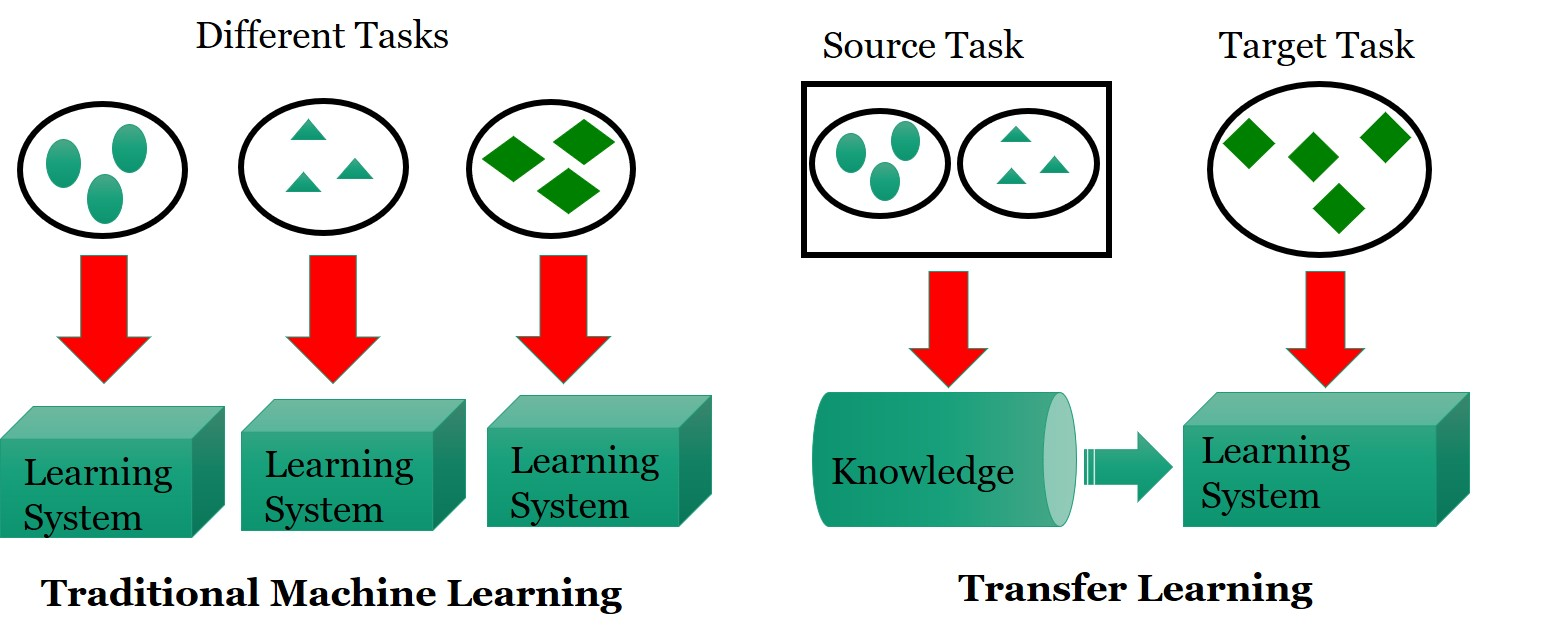
\includegraphics[width=4in,height=2in]{figures/TLGL}
%	\linebreak
%	\captionof{figure}{Conventional machine vs. transfer learning. Originally shown in~\cite{5288526}.}
%	\label{fig1:TLGL}
%\end{center}
%\end{figure}
\noindent
\enquote{What to transfer} sees which pieces of information can be transferred from one task or domain to another. Some information can be specific to a certain task or domain, and some information can be common across tasks or domains. After getting the information that can be transferred, different algorithms had been developed to deal with \enquote{how to transfer} the information. \enquote{When to transfer} figures out the criteria when transferring skills should be done. 
Transfer learning is categorized into three groups according to the labels availability in the source and target domains, and the tasks of the two domains. It is further discussed below.
\subsection{Inductive Transfer Learning}
In inductive transfer learning source and target tasks are different, and it does not matter source, and target domains are similar or different. In this case, labeled data in the target domain is required for induction. Based on the situation of labeled and unlabeled source domain, inductive transfer learning can further categorize in two cases.%\\

\noindent
\textbf{Multi-Task Learning.~}
In multi-task learning source and target tasks are learned simultaneously, it does not matter that the source and target domains are similar or different. The aim is to achieve high performance in the target task.%\\

\noindent
\textbf{Self-Taught Learning.~}
In self-taught-learning the source and target domains may have different label spaces, which show that we can not use directly side information of source domain.

\subsection{Transductive Transfer Learning}
The transductive transfer learning proposed by~\cite{arnold2007comparative}. For transductive transfer learning source and target tasks should be similar, but the domains can be different. Domain adaptation is a type of transductive transfer learning. In domain adaptation, source domain contains abundant labeled data while the target domain contains no labeled data, and the source and target domains are different. Different transductive transfer learning had been proposed. Structural Correspondence Learning (SCL) is one of them. The SCL was proposed for speech tagging. It uses the unlabeled target domain for reducing the domain data differences. Based on unlabeled data in both domains, the set of pivotal features are defined. These defined pivotal features are used to learn the mapping between original feature space and shared low-dimension feature space.
\subsection{Unsupervised Transfer Learning}
Unsupervised transfer learning is more focused to clustering, dimension reduction, where there is no need for labeled data in both source and target domains, while it is similar to multi-task learning where the source and target tasks are different but related to each other.\\


	\chapter{Methodology}
\label{methods}
%\pagenumbering{arabic} 
In this section, we discuss our novel framework implementation and also discuss different methods which are used in our framework. Our framework is based on three steps. In the first step, visual descriptors are extracted from videos using Improved Dense Trajectory method (IDT)~\cite{wang2013action}. Second, Gaussian Mixture Model (GMM) and Fisher Vector are used for feature representation. In the last, we jointly learn the dictionary and projection matrix via transfer learning to get the discriminative and transferable features for cross-view action recognition. The Joint Dictionary and Transfer Learning (JDTL) framework is an iterative process. First, the new projection matrix is obtained by using different transfer learning methods, then a dictionary is learned by fixing the projection matrix and coefficients, and finally coefficients are learned by fixing the projection matrix and updated dictionary.

\section{Feature Extraction}
The first step of our framework is to extract the features from videos. Improved Dense Trajectories (IDT) is a state-of-the-art method used for feature extraction in our study. In brief, IDT was introduced by Wang et al.~\cite{wang2013action} and is extended from dense trajectories~\cite{wang2013dense,bilinski2014human}. Dense Trajectory densely sample the feature points in video frame and track those detected features points in upcoming video frames, while IDT improves dense trajectories by explicitly estimating camera motion. %\\

\noindent
\textbf{Dense Trajectories (DT). }
It is difficult to determine the best scale to track feature points, and therefore dense trajectories are extracted from multiple spatial scales. Feature points are sampled in each frame of a video on a grid spaced by ${W}$ pixels. To obtain enough dense trajectories and catch significant motion information, the parameter $W$ is set to 5 pixels. Once feature points are extracted, these are tracked in each video frame in each spatial scale separately. Eight spatial scales are used, and each spatial scale is increased by a factor of  $\frac{1}{\sqrt{2}}$. 

Dense optical flow field $w_{t}$ is computed from frame $I_{t}$ to the following frame $I_{t+1}$, using the Farneback algorithm~\cite{farneback2003two}. Each point $P_{t} = (x_{t}, y_{t})$ at frame $t$ is tracked to the next frame $t+1$ by median filtering in dense optical flow field $w_{t} = (u_{t}, v_{t})$, where $u_{t}$, and $v_{t}$ are the horizontal and vertical components of optical flow respectively. 
\begin{equation}
\begin{aligned}
P_{t+1}\ =\ (x_{t+1},\ y_{t+1})\ =(x_{t},\ y_{t})\ +\ (M\ast\ w)\ |_{(\bar{x}_t,\ \ \bar{y}_t)}\ 
\end{aligned}
\end{equation}

\noindent
\textbf{DT Descriptors: Trajectory shape, HOG, HOF, and MBH. }
Wang et al.~\cite{wang2013action} proposed the trajectory shape descriptor to encode a form of the extracted dense trajectories. A sequence of displacement vectors normalized by the sum of displacement vectors magnitudes describe the trajectory shape.

In a space-time volume around a trajectory, three descriptors (HOG, HOF, and MBH) are calculated. Each local volume is subdivided into a grid with $ n_{x} \times n_{y} \times n_{t}$ spatio-temporal cells in order to embed structure information. A histogram descriptor is calculated for each cell of the grid. The histograms are normalized with $L_{2}$ norm, and then normalized cells are concatenated into the final descriptors. 

Similarly, the HOG and HOF descriptors are calculated for spatio-temporal interest points. In this case, edge and optical flow orientations are quantized into 8 bins using full orientations, with the HOF descriptor having an additional zero bin. The example of HOG is shown in Figure~\ref{fig:HOG-Example}, where in (a) the image is the input image, (b) input image with extracted HOG features at different locations on input image, and in (c) extracted HOG features from input image are illustrated.


 \begin{figure}[!ht]
	\centering
	\includegraphics[width=.55\textheight]{figures/HOG-final2}
	\linebreak
	\caption{(a) Input image. (b) HOG features extracted from the image at different locations. (c) HOG features illustration.}
	\label{fig:HOG-Example}
\end{figure}

Dalal et al.~\cite{dalal2006human} proposed the Motion Boundary Histogram (MBH) descriptor to detect human. Optical flow field $I_{w} = (I_{x}, I_{y})$ is separated into its $x$ and $y$ components. Spatial derivatives for the horizontal and vertical components of the optical flow field are computed separately, and the orientation information is quantized into histograms. Background motion is eliminated by suppressing the constant motion information and keeping the information about changes in the flow field.   

IDT boosts the recognition performance of dense trajectories by taking camera motion into account.\ It assumes that background motion of two consecutive frames can be characterized by a homography matrix.\ To estimate the homography matrix, the first step is to find the correspondence between two consecutive frames. They resort to SURF~\cite{bay2008} feature matching and optical flow based matching, as these two kinds of matching schemes are complementary to each other. Then RANSAC~\cite{fischler1981random} algorithm is used to estimate the homography matrix.\ Based on the homography matrix, they rectify the frame image to remove camera motion and re-calculate the optical flow called \textit{wrapped flow}. There are two major advantages for dense trajectories to cancel out camera motion from optical flow. First, this brings advantages to the descriptor calculated from optical flows, in particular for HOF. Second, trajectories generated due to camera motion can be removed.

It describes the deviation of orignal set of features from average distribution of features modeled by parametric generative model, 
\section{Feature Representation}
Once local features are extracted, these are used to represent actions in videos. As the length of each video is different, we refer to \textbf{Fisher Vector (FV)}, one of most efficient vector quantization method to represent each video and achieve a fixed length vector~\cite{perronnin2010improving,perronnin2007fisher}. FV is an extension of bag-of-visual word representation and its encoding represents differences between features and visual words. FV has achieved remarkable results as a global descriptor both for image classification and for image retrieval, outperforming the conventional bag-of-features approach.
Given a large set of vectors, the FV method assembles them into a high dimensional representation.
So, in the first stage diagonal covariance was used to train the Gaussian Mixture Model (GMM), and derivatives are considered with respect to gaussian mean and variance~\cite{simonyan2013fisher}. It gives the representation, which captures the average first and second order differences between the original feature and each of the GMM centers:
\begin{equation}
\begin{aligned}
\Phi_k^{(1)} & = \frac{1}{N  \sqrt[]{W_k}} \sum_{p=1}^{N}\ \alpha_p(k)\Bigg(\frac{x_p -\mu_k}{\sigma_k}\Bigg), \\
\Phi_k^{(2)} & = \frac{1}{N \sqrt[]{2W_k}} \sum_{p=1}^{N}\ \alpha_p(k)\Bigg(\frac{(x_p -\mu_k)^2}{\sigma_k^2} -1  \Bigg),
\end{aligned}
\end{equation}
where $\{w_k, \mu_k, \sigma_k\}_k$ are mixture weights, means, and diagonal covariances of GMM.  $\alpha_p(k)$ is the soft assignment weight of the $p$-th feature $x_p$ to the $k$-th Gaussian. An FV $\Phi$ is obtained by stacking the differences: $ \Phi = [{\Phi_1^{(1)},\Phi_1^{(2)},.....,\Phi_K^{(1)},\Phi_K^{(2)} }]$. The final encoded vector shows the difference between distribution of video features and distribution fitted to the features of all training videos.
\begin{table}[h]
\centering
\caption{Details of the variables used in our method} 
\begin{tabular}{@{\extracolsep{12pt}}|c|l|}
\hline
\textbf{Variable} & \textbf{Description} \\ \hline
$P$	&  Projection Matrix           \\ \hline
$Y$	&  Training Sample            \\ \hline
$D_0$	& Shared Dictionary             \\ \hline
$D_j$	& Class-specific Dictionary            \\ \hline
$\bar{D}$	& Total Dictionary that includes class-specific and shared dictionary            \\ \hline
$X_0$	& Shared Coefficients            \\ \hline
$X_c$	& Class-Specific Coefficients             \\ \hline
$M$	&  Each Dictionary Column Mean Vector            \\ \hline
$M_0$	&  Shared Coefficient Mean Vector            \\ \hline
$M_c$	& Class-specific Coefficient Mean Vector             \\ \hline

$J$	& Input Data Matrix (Transfer Learning)             \\ \hline
%$D_s$    &  Source Domain            \\ \hline
%$D_t$	 & Target Domain            \\ \hline
$J_s$	 & Source Task  \\ \hline
$J_t$  	&  Target Task  \\ \hline
$L_t$		& Target Label            \\ \hline
$L_s$		& Source Label            \\ \hline
$I$	& Identity Matrix             \\ \hline
%$m,c$	& Shared Feature/Classes             \\ \hline
$M_d$	& Maximum Mean Discrepancy (MMD) Matrix             \\ \hline
$M_{d_c}$ & Maximum Mean Discrepancy (MMD) Matrices involving class labels \\ \hline
$K$	& Input Kernel Parameter             \\ \hline
%$\phi$	& Feature Map induced by Kernel             \\ \hline
$\mathcal{P}$	&  Marginal Distribution           \\ \hline	
$\mathcal{Q}$	&  Conditional function           \\ \hline
$H$	&  Centering Matrix           \\ \hline	
$\triangleq$ & equal by definition \\ \hline	
$\mu ,\lambda$	&  Trade-off Parameter/Regularize parameter\\ \hline		
\end{tabular}
\label{tb:TLVariable}
\end{table}
\noindent
\section{Transfer Learning}
Transfer learning is employed in this chapter to map the source (one view) and target (another view) features into a common subspace. The transfer learning methods are categorized in supervised, semi-supervised and unsupervised as we described in related work, and we detail four methods below which will be incorporated into the joint learning framework. The variables and  basic formulation in this chapter can be found in Table~\ref{tb:TLVariable} and~\ref{table:tcl}.
\begin{table}[h]
	\footnotesize
	%\large
	\centering
	\caption{Transfer learning methods} 
%	\resizebox{\textwidth}{!} {%
		\begin{tabular}{|m{2cm}|m{9cm}|m{2.9cm}|}
			\hline   
			Method & Learning Objective & Constraints  \\ 
			\hline
			Transfer Component Analysis&  $\min_W \textbf{tr}(W^\T W) + \mu \ \textbf{tr}(W^\T KLKW)$ &$W^\T KHKW = I$\\ \hline
			Joint Distribution Adaptation&$\min\ \sum_{C}^{c=0} \textbf{tr}(J^\T JM_{d_c}J^\T A) \ + \ \lambda ||A||_F^2 $ & $A^\T JHJ^\T A= I$           \\ \hline
			Balance Distribution Adaptation&  $\min \  \textbf{tr} \bigg(A^\T J \bigg((1-\mu )M_{d_0} \ + \mu \sum_{c=1}^{C}M_{d_c}\bigg)J^\T A \bigg)\ +\lambda||A||_F^2$&$A^\T JHJ^\T A= I$ , $0\leq \mu \leq 1$         \\ \hline
			Transfer Joint Matching & $\min \textbf{tr}(A^\T KM_dK^\T A)\ +\lambda \big(||A_s||_{2,1} + ||A_t||_F^2 \big)$ &$A^\T KHK^\T A= I $           \\  \hline
			%\hline
		\end{tabular}%
%	}
	\label{table:tcl}
\end{table}

\subsection{Transfer Component Analysis}
The Transfer Component Analysis (TCA) algorithm reduces marginal distribution difference using a Reproducing Kernel Hilbert Space to discover common latent features~\cite{pan2011domain,8258419}. The Maximum Mean Discrepancy (MMD) measure is used to determine the marginal distribution difference between the source and target data. The TCA optimization equation is given in Table~\ref{table:tcl} where $\mu$ is the trade-off parameter, $I$ is the identity matrix, $H$ is the centering matrix, $K$ is the kernel matrix. As transform matrix should not collapse at one point, an additional non-convex term constraint is added $W^\T KHKW = I$ to inflates the kernel. Therefore, the embedded data is preserved.

\subsection{Transfer Joint Matching}
The Transfer Joint Matching (TJM) algorithm aims to reduce the marginal distribution difference by first performing a dimensionality reduction step using Principal Component Analysis (PCA). Next, the MMD measure is employed in a Reproducing Kernel Hilbert Space to perform the feature matching method. At last, with the help of instance reweighing irrelevant instances are reduced and distribution difference is further minimized~\cite{6751384}.
The TJM jointly match features and reweigh the source instances to reduce the domain differences. The formulation of TJM is given in Table~\ref{table:tcl}, where ${A, K, M_d}$ are the adaptation matrix, kernel matrix, and MMD measure respectively, while $l_{2,1}$ sparsity constraint is added as a sparsity regularizer on the transformation matrix. Additional constraint $A^\T KHK^\T A = I$ is imposed to ensure that transform data should not collapse at one point.
\subsection{Joint Distribution Adaptation}
The Joint Distribution Adaptation (JDA) algorithm attempts to simultaneously correct the marginal and conditional distribution differences between the source and target data. The MMD distance measure is integrated into the PCA algorithm, which is used as a dimensionality reduction step to correct the marginal distribution differences. Pseudo labels are predicted by learning a classifier from the labeled source data, which are used to improve the conditional distribution differences~\cite{6751384}. The formulation of JDA algorithm is given in Table~\ref{table:tcl}, where $J$ is input data, $A$ is transformation matrix, $M_{d_c}$ is MMD matrices involving class labels, $A$ is the adaptation matrix and $\lambda$ is the regularization parameter to ensure that the optimization problem should be well-defined. 
\subsection{Balanced Distribution Adaptation}
Balanced Distribution Adaptation (BDA) is proposed to balance the marginal and conditional distribution when marginal distribution becomes more dominant when datasets are very different and conditional distribution becomes more important for more similar datasets. Most of the transfer learning methods assume that data is balanced, but the imbalanced data widely exists in real issues. The class imbalance is handled by introducing Weighted Balanced Distribution Adaptation(W-BDA) algorithm, which adjusts the weight of each class in addition to the adaptation of distribution~\cite{wang2017}.
The formulation of BDA is given in Table~\ref{table:tcl}. Where $J$ is the input data, $A$ represents transformation matrix, $I$ denotes an identity matrix, $H$ is the centering matrix and $M_{d_0}$ and $M_{d_c}$ are MMD matrices. 
The equation is divided into two terms, term 1 is the adaptation of marginal and conditional distribution with a balance factor, the second term is the regularization term. Two constraints are involved in BDA equation, $A^\T J$ ensures that transformed matrix should preserve the original data properties. The second constraint denotes the range of balance factor $\mu$.

\section{Dictionary Learning}
Before discussing our approach, first, we discuss the basic dictionary learning (DL) model.
In many applications, the dictionary $D$ is unknown and has to be learned from the training signals coming from the desired class. A DL algorithm finds an over-complete dictionary $D$ that sparsely represents measurement $Y$ such that $Y \simeq DX$. Each of these vectors $ x_i$ is the sparse representation of $y_i$ with only $s$ nonzero entries.
Suppose training data from different categories denoted by $X_i \in \mathbb{R}^d(i=1,...N)$. In DL we want to find a dictionary $D \in \mathbb{R}^{d \times K} $ and a coefficient matrix 
$X = [x_i,.... x_N] \in \mathbb{R}^{K \times N}$, such that both $D$ and $X$ are minimized and the representations $X$ are sparse enough. A non-traceable formulation of this problem is 
\begin{equation}
\begin{aligned}
& \underset{D,X} \min ||Y-DX||_F^2 \\
\text{subject to } &  ||x_i||_0 \leqslant s, 1 \leqslant i \leqslant L,
\end{aligned}
\label{eq:DL1}
\end{equation}
\noindent
where $\|\|_0$ means vector $\ell_0$ norm.
Since both $D$ and $X$ are unknown, a common approach is to use alternating minimization in which we start with an initial guess of $D$ and then obtain the solution iteratively by alternating between two stages, sparse coding and dictionary update. The flow of dictionary learning is shown in Figure~\ref{fig1:DLSC}.
\begin{figure}[!ht]
\centering
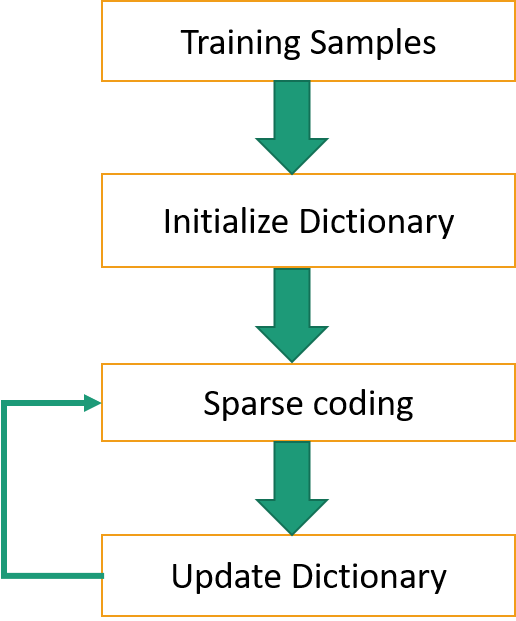
\includegraphics[width=.22\textheight]{figures/DLpipeline}
\linebreak
\caption{Pipeline of basic dictionary learning and sparse coding.}
\label{fig1:DLSC}
\end{figure}

\section{Joint Transfer and Dictionary Learning Framework}

The JDTL paradigm is shown in Figure~\ref{fig1:JLP}. The left-hand side of the figure is the generic transfer learning modeling where different views features are brought into common subspace using different transfer learning methods. While on the right-hand side we aim to learn view independent dictionary and coefficients by using the LRSDL~\cite{7987024} method. More detail is given in following subsections.

\begin{figure}[!ht]
	\centering
	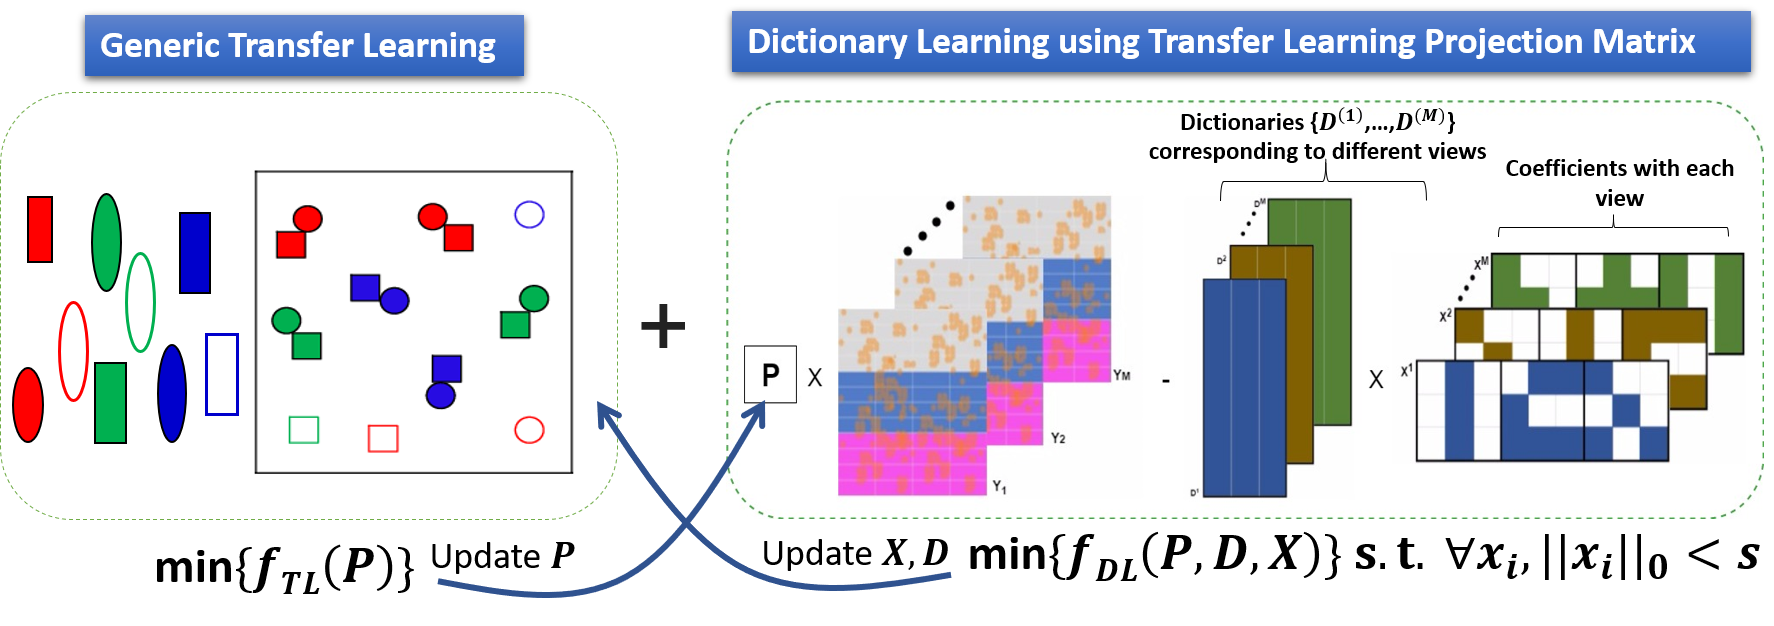
\includegraphics[width=.66\textheight]{figures/JLPara2}
	\linebreak
	\caption{Joint dictionary and transfer learning paradigm.}
	\label{fig1:JLP}
\end{figure}
\begin{figure}[!ht]
	\centering
	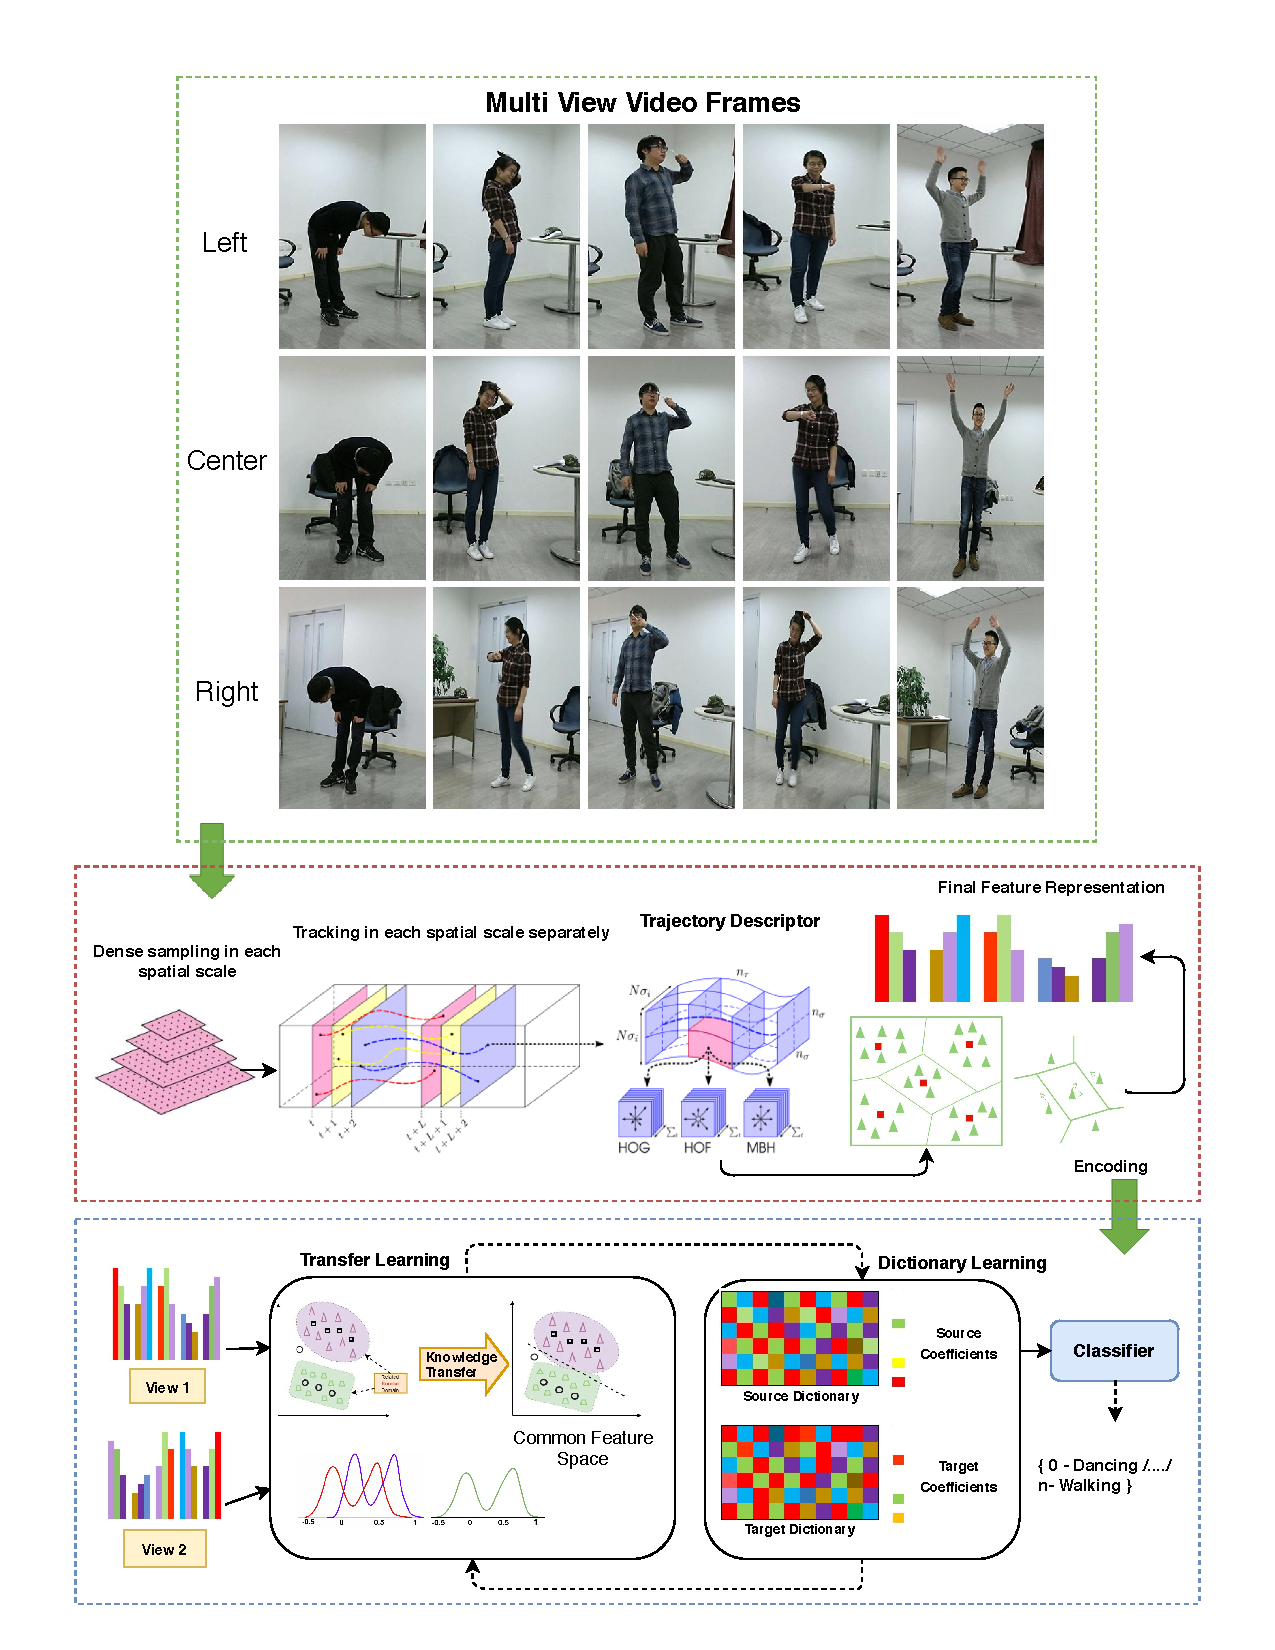
\includegraphics[width=.66\textheight]{figures/framework/updatewholepage2}
	\linebreak
	\caption{Overview of the proposed joint learning objective. Part of illustration is from~\cite{HengWang:2011:ARD:2191740.2192078}.}
	\label{fig1:JDTL}
\end{figure}
\subsection{Framework Overview}
The framework of our proposed method is shown in Figure~\ref{fig1:JDTL}. Where first we extract features from videos of each view using IDT method, then different transfer learning methods are used to bring features from different views into common subspace, and transfer learning projection matrix is learned. After learning the projection matrix, the view independent dictionary is learned. In the last, our novel approach is used to jointly learn the dictionary and projection matrix in order to get the optimized dictionary, coefficients and transfer learning projection matrix. Finally, SVM is used for the classification.

\subsection{Model Construction}
Let $Y$ be a set of $m$-dimensional training samples, i.e., $Y^{(v)} = [Y_1^{(v)}, Y_2^{(v)}, ....., Y_C^{(v)}]$ where $Y_i$ denotes the training sample from class $i$ and $C$ denotes the number of classes for each view. The view independent dictionary is denoted by $D^{(v)}= [D_1^{(v)}, D_2^{(v)},....,D_C^{(v)}]$ where $D_i$ is sub-dictionary associated with class $i$ and $v$ represents the views. In this approach we also learn the transfer learning projection matrix $P \in R^{m\times d}$, that projects the data into lower-dimensional space. $X^{(v)}$ is the sparse representation matrix of dimensionality reduced data $P^\T Y$ over dictionary $D^{(v)}$,
$f_{\text{TL}}(\cdot)$ is the transfer learning objective function which we get from different transfer learning methods, $f_{\text{DL}}(\cdot)$ is the general dictionary learning function. Hence, our proposed novel approach is given in the following equation:
\begin{equation}
\begin{aligned}
%\underset{D,X,P} \min = P_tY + ||P_{t-1}Y - D_{t-1}X_{t-1} ||
% & \min f(P) + ||P^\T Y - DX ||_F^2, \\
& \min_{P,D,X} f_{\text{TL}}(P) + \gamma f_{\text{DL}}(P,D,X), \\
\text{s.t. } & ||x_i||_0 < s \text{ and } x_i \text { is a column of } X,
\end{aligned}
\label{label:JDLTL}
\end{equation}
where $\gamma$ is the balancing parameter.


\subsection{Optimization}
The above equation can not be solved in closed form, so we refer to an iterative solution. The iterative process is shown in Figure~\ref{fig1:novelpipeline} and Algorithm~\ref{alg:JDTL}. Here our goal is to learn the projection matrix obtained via transfer learning and in the next step based on the projection matrix dictionary and sparse codes are updated.
The objective function in Eq.~\eqref{label:JDLTL} can be divided into three subproblems, to jointly learn projection $P$, dictionary $D$ and coding coefficients $X$.

\begin{figure}[!ht]
	\centering
	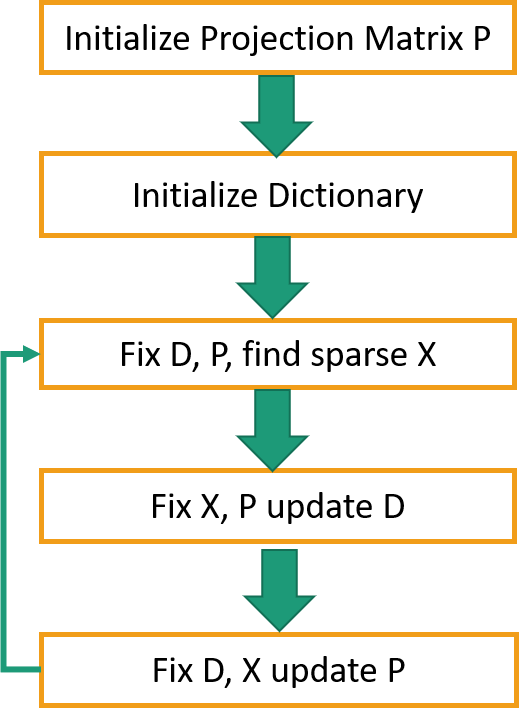
\includegraphics[width=.22\textheight]{figures/novelpipeline}
	\linebreak
	\caption{Pipeline of joint dictionary and transfer learning.}
	\label{fig1:novelpipeline}
\end{figure}  
\begin{algorithm}
	\caption{Joint Dictionary and Transfer Learning}
	\begin{algorithmic}[1]
		\State \textbf{Input}\\
		~~~Initialize $P_i$ as an output from transfer learning method.\\
		~~~Initialize $D_i$ and $X_i$ as a view independent Dictionary and Coefficients respectively 
		\While{convergence or maximal iteration step is not reached}
		\State $t \leftarrow t+1$
		\State Fix $P_i$ and $D_i$, update $X_i$  using \textbf{Equation:~\eqref{eq:DLX}}
		\State Fix $P_i$ and $X_i$, update $D_i$ using \textbf{Equation:~\eqref{eq:DL0}}
		\State Fix $D_i$ and $X_i$, update $P_i$  using \textbf{Equation:~\eqref{eq:DLPL}}
		\EndWhile\label{euclidendwhile}
		\State \textbf{output} $P, X$ and $D$
	\end{algorithmic}
\label{alg:JDTL}
\end{algorithm}
\noindent

First, different transfer learning methods are used to get the projection matrix. The projection matrix is learned by calculating the gradient of the projection matrix. Fast Low-Rank Shared Dictionary Learning (LRSDL) framework is used for the dictionary and coefficient learning. LRSDL method automatically extracts both discriminative and shared bases. LRSDL framework is a supervised method which learns a dictionary to extract the discriminative features for each class independently and also learns the shared features~\cite{7987024}. In our method shared dictionary and coefficients are used. FDDL has been broadly used for exploiting both structured dictionary and learning discriminative coefficient in LRSDL~\cite{612628612}. Specifically, the discriminative dictionary $D$ and the sparse coefficient matrix $X$ is learned based on the following equation.
\begin{equation}
\begin{aligned}
	J_Y(D,X) = \frac{1}{2}f_Y(D,X) + \lambda_1||X||_1 + \frac{\lambda_2}{2}g(X),
\end{aligned}
\label{eq:DL}
\end{equation}
where $f_Y(D,X) =  \sum\limits_{c=1}^{C} r_{Y_c}(D,X_c)$ is a discriminative fidelity with:
\begin{equation}
\begin{aligned}
r_{Y_c}(D,X_c) = ||Y_c-DX_c||_F^2 + ||Y_c - D_cX_c^c||_F^2 + \sum\limits_{j\neq c}||D_jX_c^j||_F^2.
\end{aligned}
\end{equation}

For $c = 1, \cdots,C$ ; $i =0,1,\cdots, C$. Assume that $Y_c \in \mathbb{R}^{d\times n_c}$ and $Y \in \mathbb{R}^{d \times N}$ with $N = \sum_{c=1}^{C}n_c$; $D_i \in \mathbb{R}^{d\times k_i} , D \in \mathbb{R}^{d\times K}\text{ with } K = \sum_{c=1}^{C}k_c $; and $X \in \mathbb{R}^{K \times N}$. Notation $X^i$ means the sparse coefficient of $Y$ on $D_i$, by $X_c \in \mathbb{R}^{K \times N_c}$ means the sparse coefficient of $Y_c$ on $D$ and by $X_c^i$ means the sparse coefficient of $Y_c$ on $D_i$.  

The last term in $r_{Y_c}(D,X_c)$ means that $D_j$ has small contribution to the representation of $Y_c$ for all $j\neq c$, and $g(X) = \sum_{c=1}^{C}(||X_c - M_c||_F^2 - ||M_c - M||_F^2) + ||X||_F^2 $. In $g(X)$, 
$M_c = \mu(X_c)$ and $M = \mu(X,n)$ is the mean matrices. $n$ is the number of columns depending on the context. The last term $||X||_F^2$ in $g(X)$ makes the cost function convex with respect to $X$. These subproblems are optimized alternatively by updating one variable and fixing the others, through an iterative process. Our proposed method is discussed in the following sections.

\subsection*{Updating Coding Coefficients $X$}

Assuming $D$ and $P$ are fixed, $X$ is solved by following equation:
\begin{equation}
\begin{aligned}
\min_X h(X) + \lambda ||X||_1,
\end{aligned}
\label{eq:DLX}
\end{equation}
where $h(X) = \frac{1}{2}f_{Y,D}(X) + \frac{\lambda_2}{2}g(X)$. This problem can be solved by FISTA~\cite{beck2009fast}. Where gradient of $f(\cdot)$ and $g(\cdot)$ are calculated with respect to $X$.
%Where we need to calculate gradient of $f(\cdot)$ and $g(\cdot)$ with respect to $X$. 
The gradient of $h(X)$ is calculated in FDDL method by the following equation: 
\begin{equation}
\begin{aligned}
\frac{\partial \frac{1}{2}f_{Y,D}(X)}{\partial X} = \mathcal{M}(D^\T D)X - \mathcal{M}(D^\T Y),
\end{aligned}
\label{eq:GRAD1}
\end{equation}
\begin{equation}
\begin{aligned}
\frac{\partial \frac{1}{2}g(X)}{\partial X} = 2X + M -2\underbrace{[M_1, M_2 ,.... , M_c]}_{\widehat{M}},
\end{aligned}
\label{eq:GRAD21}
\end{equation}
Where $\mathcal{M(\cdot)}$ doubles the diagonal block of the given matrix. The row and column partition of the matrix are inferred from the given matrix and it is also computationally inexpensive function of the given matrix . $\widehat{M}=[M_1, M_2 ,.... , M_c] = [\mu(X_1), \mu(X_2) ,.... , \mu(X_c)]$ is the mean of each class specific coefficients.

\noindent
Using Eq.~\eqref{eq:GRAD1} and Eq.~\eqref{eq:GRAD21} we obtain:
\begin{equation}
\begin{aligned}
\frac{\partial h(X)}{\partial X} = (\mathcal{M} (D^\T D) + 2 \lambda_2 I)X - \mathcal{M}(D^\T Y)+\lambda_2(M-2 \widehat{M}).
\end{aligned}
\label{eq:GRAD2}
\end{equation}

As the LRSDL is the extension of FDDL, class-specific coefficients $X$ and shared coefficients $X^0$ are solved alternatively, Here $X$ and $X^0$ are combined into one and find $\bar{X}$ by solving the following optimization problem:%  and will solve the optimization problem by the following equation:
\begin{equation}
\begin{aligned}
\bar{X} = \mathrm{arg}\ \underset{\bar{X}}{\min}\ {\bar{h}(\bar{X})} + \lambda_1 ||\bar{X}||_1.
\end{aligned}
\label{eq:GRAD3}
\end{equation}
where $\bar{h}(\bar{X}) = \frac{1}{2} \bar{f}_{Y,\bar{D}}(\bar{X}) + \frac{\lambda_2}{2}\bar{g}(\bar{X})$. This problem is solved using FISTA with the gradient of $\bar{h}(\bar{X})$:
\begin{equation}
\begin{aligned}
\bigtriangledown \bar{h}(\bar{X}) = 
\begin{bmatrix} \frac{\partial \bar{h}_{X^0}(X)}{\partial X} \\ \frac{\partial \bar{h}_{X}(X^0)}{\partial X^0} \end{bmatrix}.
\end{aligned}
\label{eq:GRAD4}
\end{equation}
\noindent
In the upper term, by combining the observations
\begin{equation}
\begin{aligned}
\bar{h}_{X^0}(X) & = \frac{1}{2}\bar{f}_{Y, \bar{D},X^0} (X) + \frac{\lambda_2}{2}\bar{g}_{X^0}(X)\\
& = \frac{1}{2}\bar{f}_{\bar{Y},{D}} (X) + \frac{\lambda_2}{2}{g}(X) + \text{constant},
\end{aligned}
\label{eq:GRAD5}
\end{equation}
where $\bar{D} = [D D_0]$ is total dictionary  and $\bar{Y} = Y - D_0X^0$ 
and using the equation, we have:
\begin{equation}
\begin{aligned}
\frac{\partial \bar{h}_{X^0}(X)}{\partial X} = (\mathcal{M} (D^\T D) + 2 \lambda_2 I)X - \mathcal{M}(D^\T \bar{Y})+\lambda_2(M-2 \widehat{M}).
\end{aligned}
\label{eq:GRAD6}
\end{equation}
the lower term is solved by 
\begin{equation}
\begin{aligned}
\bar{h}_X(X^0) = ||V-D_0X^0||_F^2 + \frac{\lambda_2}{2}||X^0 - M^0||_F^2 + \text{constant},
\end{aligned}
\label{eq:GRAD7}
\end{equation}
\begin{equation}
\begin{aligned}
\Rightarrow \frac{\partial \bar{h}_{X}(X^0)}{\partial X^0} & = 2D_0^TD_0X^0 - 2D_0^TV +\lambda_2(X^0 - M^0),\\
& = (2D_0^TD_0+\lambda_2I)X^0 - 2D_0^TV - \lambda_2M^0,
\end{aligned}
\label{eq:GRAD8}
\end{equation}
where $V = Y-\frac{1}{2}D\mathcal{M}(X)$ and $X^0$ is the shared coefficients and $M^0$ is the mean vector of shared coefficients. The Eq.~\eqref{eq:GRAD4} can be solved by combining Eq.~\eqref{eq:GRAD8} and Eq.~\eqref{eq:GRAD6}.
%So combining Eq.~\eqref{eq:GRAD8} and~\eqref{eq:GRAD6}, the Eq.~\eqref{eq:GRAD4} can be solved.
After solving the equation, $\bigtriangledown \bar{h}(\bar{X})$, $\bar{X}$ can be updated by FISTA algorithm. We also need to compute the Lipschitz coefficient $L$ of $\bigtriangledown \bar{h}(\bar{X})$.


\subsection*{Updating Dictionary $D$}

$D$ is updated by fixing $P$ and $X$. 
The most important part of the shared dictionary is to represent samples from all classes. In other words,
it is expected that the collaboration of the particular dictionary $D_c$ and the shared dictionary $D_0$ should well represent $Y_c$. 
 %it is expected that $Y_c$ can be well represented by the collaboration of the particular dictionary $D_c$ and shared dictionary $D_0$. 
 The discriminative fidelity term $f_Y(D,X)$ in Eq.~\eqref{eq:DL} can be extended to $\bar{f}_Y(\bar{D},\bar{X}) = \sum_{c=1}^{C}\bar{r}_{Y_c}(\bar{D},\bar{X_c})$ with $\bar{r}_{Y_c}(\bar{D},\bar{X_c})$ is defined as:
%This above approach can be solved by the following equation:
\begin{equation}
\begin{aligned}
||Y_c-\bar{D}\bar{X_{c}}||_F^2 + ||Y_c-D_c X_c^c-D_0X_c^0||_F^2 + \sum_{j=1,j\neq c} ||D_jX_c^j||_F^2.
\end{aligned}
\label{eq:DL0}
\end{equation}
Since $\bar{r}_{Y_c}(\bar{D},\bar{X_c}) = r_{\bar{Y}_c}(D,X_c)$ with $\bar{Y}_c = Y_c-D_0X_c^0$, we have $\bar{f}_Y(\bar{D},\bar{X}) = f_{\bar{Y}}(D,X)$ with $\bar{Y}=Y-D_0X^0$

The atoms that are the part of shared dictionary $D_0$ should represent the samples from all classes. The nuclear norm regularization $||D||_*$ is used as a convex relaxation of $D_0$. It forces that shared dictionary should have low-rank to prevent the dictionary from absorbing the discriminative atoms and it handles the worst case, where all atoms are the part of shared dictionary and there is no discriminative features remaining for class-specific atoms.

The contribution of each class-specific feature might be different, even the shared dictionary has low-rank. The contribution of each class-specific feature is measure by shared coefficients $X_0$, which they aim to avoid. A regularization term $||X^0 - M^0||$ is added that forces each $x^0$ to be close to mean vector $m^0$ for all $X^0$. By adding this constraint, the fisher-based discriminative coefficient term $g(x)$ can be extended to $\bar{g}(\bar{x})$ and it is defined as:
\begin{equation}
\begin{aligned}
	\bar{g}(\bar{x}) = g(X) +||X^0-M^0||_F^2,
	\end{aligned}
	\label{extendg(x)}
\end{equation}
In total, the cost function $\bar{J}_Y(\bar{D},\bar{X})$ of the LRSDL method is: 
\begin{equation}
\begin{aligned}
\bar{J}_Y(\bar{D},\bar{X}) = \frac{1}{2}\bar{f}_Y(\bar{D},\bar{X})+\lambda_1||\bar{X}||_1 + \frac{\lambda_2}{2}\bar{g}(\bar{X}) + \eta||D^0||_*.
\end{aligned}
\label{lrsdlcostfunction}
\end{equation}
The shared dictionary and class-specific dictionary can be found by minimizing the objective function. $\bar{D}, \bar{X}$ become $D, X$ respectively, $\bar{J}_Y(\bar{D},\bar{X})$ becomes $J_Y({D},{X})$ and LRSDL reduces to FDDL in case if there is no shared dictionary.

The FDDL method updates each class-specific dictionary by fixing the $X$. This process takes time for convergence, so in LRSDL the total dictionary $D$ is optimized while fixing $X$ instead of updating the class-specific dictionaries, so this problem is given in below equation:
\begin{equation}
\begin{aligned}
\min_D \ f_{Y,X}(D) \Rightarrow \min_D\big\{-2 \textbf{tr}(ED^\T) +\textbf{tr}(FD^\T D)\big\},
\end{aligned}
\label{eq:DL1}
\end{equation}
where $E= Y \mathcal{M}(X^\T) $, \textbf{tr($\cdot$)} means the trace of a matrix, and \textcolor{blue}{${F}$}$ = \mathcal{M}(XX^\T)$.

The LRSDL method finds total dictionary $\bar{D} = [D, D_0]$. So, the method solves the $D$ and $D_0$ separately. First, to update the $D$ in Eq.~\eqref{eq:DL0}, assuming $\bar{f}_y(\bar{D}, \bar{X}) = f_Y(D,X) $ with $\bar{Y} \triangleq Y_ {D_0}X^0$, the E-FDDL-D algorithm for $D$ is similar to Eq.~\eqref{eq:DL1}. Second, $D_0$ is optimized through the following equation when $D, X$ in Eq.~\eqref{lrsdlcostfunction} are fixed,
\begin{equation}
\begin{aligned}
\bar{J}_{Y,D,X}(D_0,X_0) = & ||V-D_0X_0||_F^2 + \frac{\lambda_2}{2} ||X^0 - M^0||_F^2 + \\ 
 & \eta||D_0||_* + \lambda_1||X^0||_1 + \text{constant},\\
\end{aligned}
\label{eq:DL4}
\end{equation}
and $V = Y- \frac{1}{2}D\mathcal{M}(X)$. 
The $D_0$ is updated by solving following equation based on the above equation:
\begin{equation}
\begin{aligned}
\min_{D_0} \ \textbf{tr}(FD_0^\T D_0) -2 \textbf{tr}(ED_0^\T)+ \eta ||D_0||_*,
\end{aligned}
\label{eq:DL5}
\end{equation}
where $E=V(X^0)^T$ ; $F = X^0(X^0)^T$ using the ADMM~\cite{boyd2011distributed36} method and singular value thresholding algorithm~\cite{cai2010singular}. In ADMM process we choose $\rho$ that should be greater than 0 and $Z = U = D_0$ is initialized, then the following problems are solved alternatively until they meet convergence.
\begin{equation}
\begin{aligned}
& \min_{D_0} - 2\textbf{tr}(\bar{E}D_0^\T) + \textbf{tr}(\bar{F}D_0^\T D_0), \\
& \text{with }\bar{E} = E+\frac{\rho}{2}(Z-U);  \bar{F} = F+\frac{\rho}{2}I,\\
\end{aligned}
\label{D0update}
\end{equation}
\begin{equation}
\begin{aligned}
Z = \mathcal{D_{\eta/\rho}}(D_c+U),
\end{aligned}
\label{Zeq}
\end{equation}
where $\mathcal{D}$ is shrinkage thresholding operator~\cite{cai2010singular}.
\begin{equation}
\begin{aligned}
U = U+D_0-Z.
\end{aligned}
\label{Ueq}
\end{equation}
The Eq.~\eqref{D0update} can be solved by ODL~\cite{mairal2010online} and the Eq.~\eqref{Zeq} and Eq.~\eqref{Ueq} are computationally inexpensive.

\subsection*{Updating Projection $P$}
First different transfer learning methods are used to get the projection matrix. Then, we minimize the projection matrix by calculating the gradient of the projection matrix. The projection matrix is optimized by using the similar way as sparse coefficients $X$ are optimized. Here, we used the FDDL method to optimize the projection matrix. 
\begin{equation}
\begin{aligned}
\min_P \frac{1}{2}f_{Y,D,X}(P) + \frac{\lambda_2}{2}g(P).
\end{aligned}
\label{eq:DLPL}
\end{equation}
This problem can be solved by FISTA, where we need to calculate gradient with respect to $P$. The gradients of the first and second terms can be calculated by FDDL method using the equations given below.   

\begin{equation}
\begin{aligned}
\frac{\partial \frac{1}{2}f_{Y,D}(P)}{\partial P} = \mathcal{M}(D^\T D)P - \mathcal{M}(D^\T (P^\T Y)),
\end{aligned}
\label{eq:PGRAD1}
\end{equation}
\begin{equation}
\begin{aligned}
\frac{\partial \frac{1}{2}g(P)}{\partial P} = 2P + M -2\underbrace{[M_1, M_2 ,.... , M_c]}_{\widehat{M}}.
\end{aligned}
\label{eq:PGRAD2}
\end{equation}
Using Eq.~\eqref{eq:PGRAD1} and~\eqref{eq:PGRAD2} we obtain:
\begin{equation}
\begin{aligned}
\frac{\partial h(P)}{\partial P} = (\mathcal{M} (D^\T D) + 2 \lambda_2 I)P - \mathcal{M}(D^\T (P^\T Y))+\lambda_2(M-2 \widehat{M}).
\end{aligned}
\label{eq:GRAD245}
\end{equation}







	
	\chapter{Experimental Setup}
\label{experimentalsetup}
%\pagenumbering{arabic} 
The performance of our method is evaluated on the PKU-MMD~\cite{liu2017pku}, a multi-view dataset. The dataset consists of 51 different classes and each action is captured from three different angles. In our experiment, we used only five action classes and multi-view videos. In PKU-MMD dataset each video contains different number of actions that requires video segmentation to segment them into individual action. The video contains multiple objects in the background and those objects are not required in our study, so a human detector is used to crop video frames. 
The detail description of the dataset, data preprocessing and experimental setup is given in this chapter.

\section{PKU-MMD Dataset}
PKU-MMD is a large-scale dataset. This dataset mainly focuses on long continuous sequences action detection and multi-modality analysis. This dataset contains 51 action classes in total. These classes are divided into two parts: 41 daily routine actions (drinking, brushing your teeth, waving hand, etc.) and 10 interaction actions (hugging, shaking hands, giving something to another person, kicking another person, etc.). 


The dataset was captured in a daily life indoor environment through Kinect sensor. Videos are captured from three different horizontal views on fixed height and angle. Horizontal angles of each camera is -45$^{\circ}$, 0$^{\circ}$, and +45$^{\circ}$ with the height of 120 \si{cm}.
The dataset was collected by 66 distinct subjects, each subject took part in 4 daily-life actions and 2 interactive actions. Figure~\ref{fig1:PKUMMD} represents PKU-MMD dataset where different actions are performed in different views by different subjects.
\begin{figure}[!ht]
	
	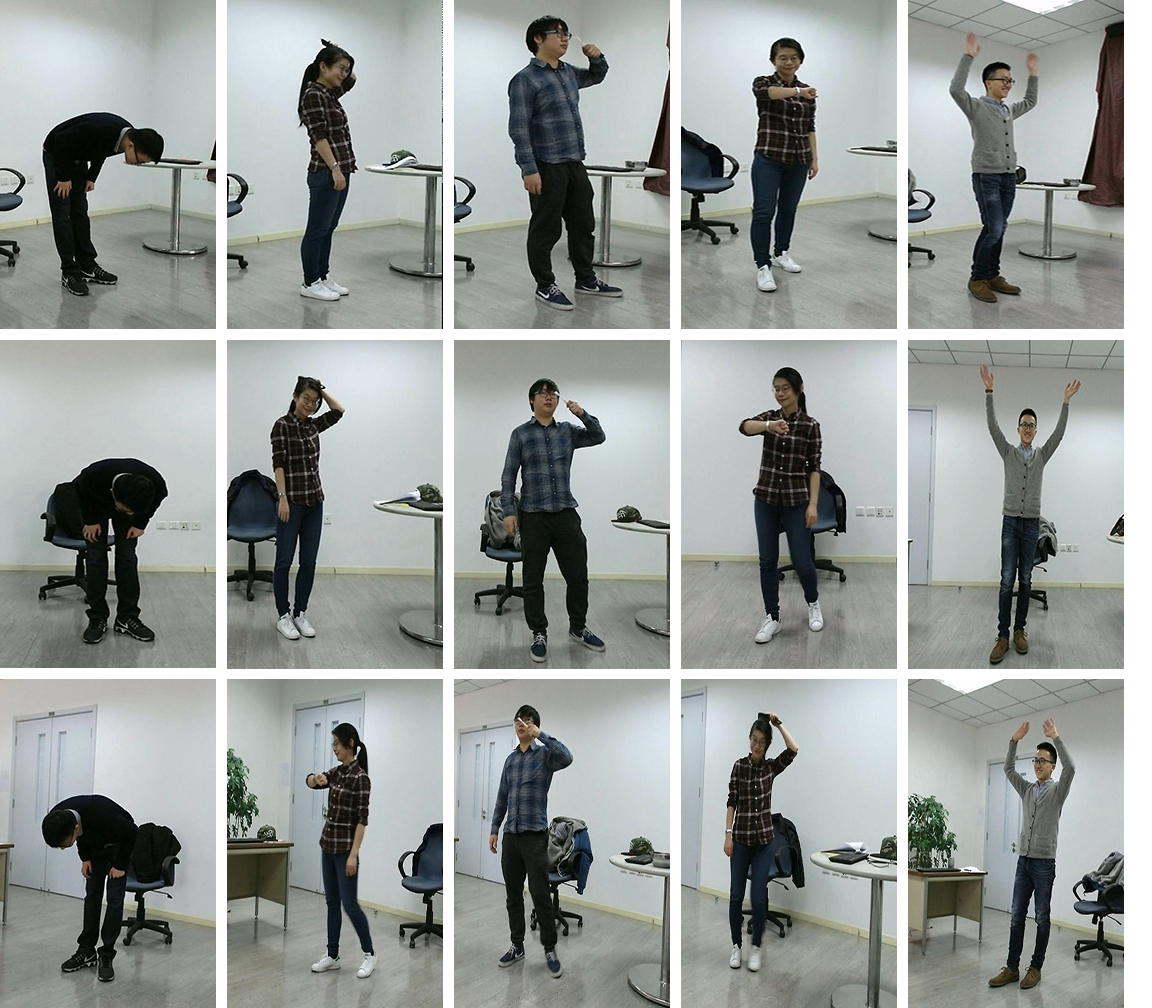
\includegraphics[width=6in,height=4in]{figures/PKUMMD-NEW1}
	\linebreak
	\captionof{figure}{PKU-MMD video sample frames from three different angles.}
	\label{fig1:PKUMMD}
\end{figure}
\section{Data Preprocessing} 
The data preprocessing consist of two steps. In the first step, large videos containing multiple actions are segmented into smaller videos which contain only a single action. Then an object detector is used to detect humans and other objects in video frames. The object detector also gives the bounding box information and based on that information video frames are cropped to remove the background objects, which are not required for the study.
\subsection{Data Segmentation}

The dataset has 1000+ long action sequences, each of which lasts about 3$\sim$4 minutes and has about 20 action instances. For each long action sequence, the data label file is provided that contains the label information for each action in video and the starting and ending frame of an action. Based on the label file information, each video is segmented. After segmenting each view, the dataset has 3,000 minutes video with 20,000+ temporally localized actions. 
\subsection{Video Frame Cropping}

The PKU-MMD dataset is collected through Kinect V2 sensor with a resolution of $1920\times1080$ pixels. While the action setup area is 180 \si{cm} as length and 120 \si{cm} as width. To crop the images, we have to first detect the person in the frame and based on that we have to crop the frames. For the person detection, we used YOLO (You Only Live Once)~\cite{DBLP:journals/corr/RedmonF16} the state-of-the-art, real-time object detection system that can detect over 9000 objects. 

The YOLO does not only detect objects in the video frame, but also labels them as shown in Figure~\ref{fig1:PKUMMD-Example}. It outputs the bounding box positions for each frame. So, in our method, we first used YOLO to detect the person in videos and get the bounding box values for the detected person in each frame. Then, single maximum bounding box value is chosen from all video frames and based on the maximum bounding box size for a person of all videos.
\begin{figure}[!ht]
	\centering
	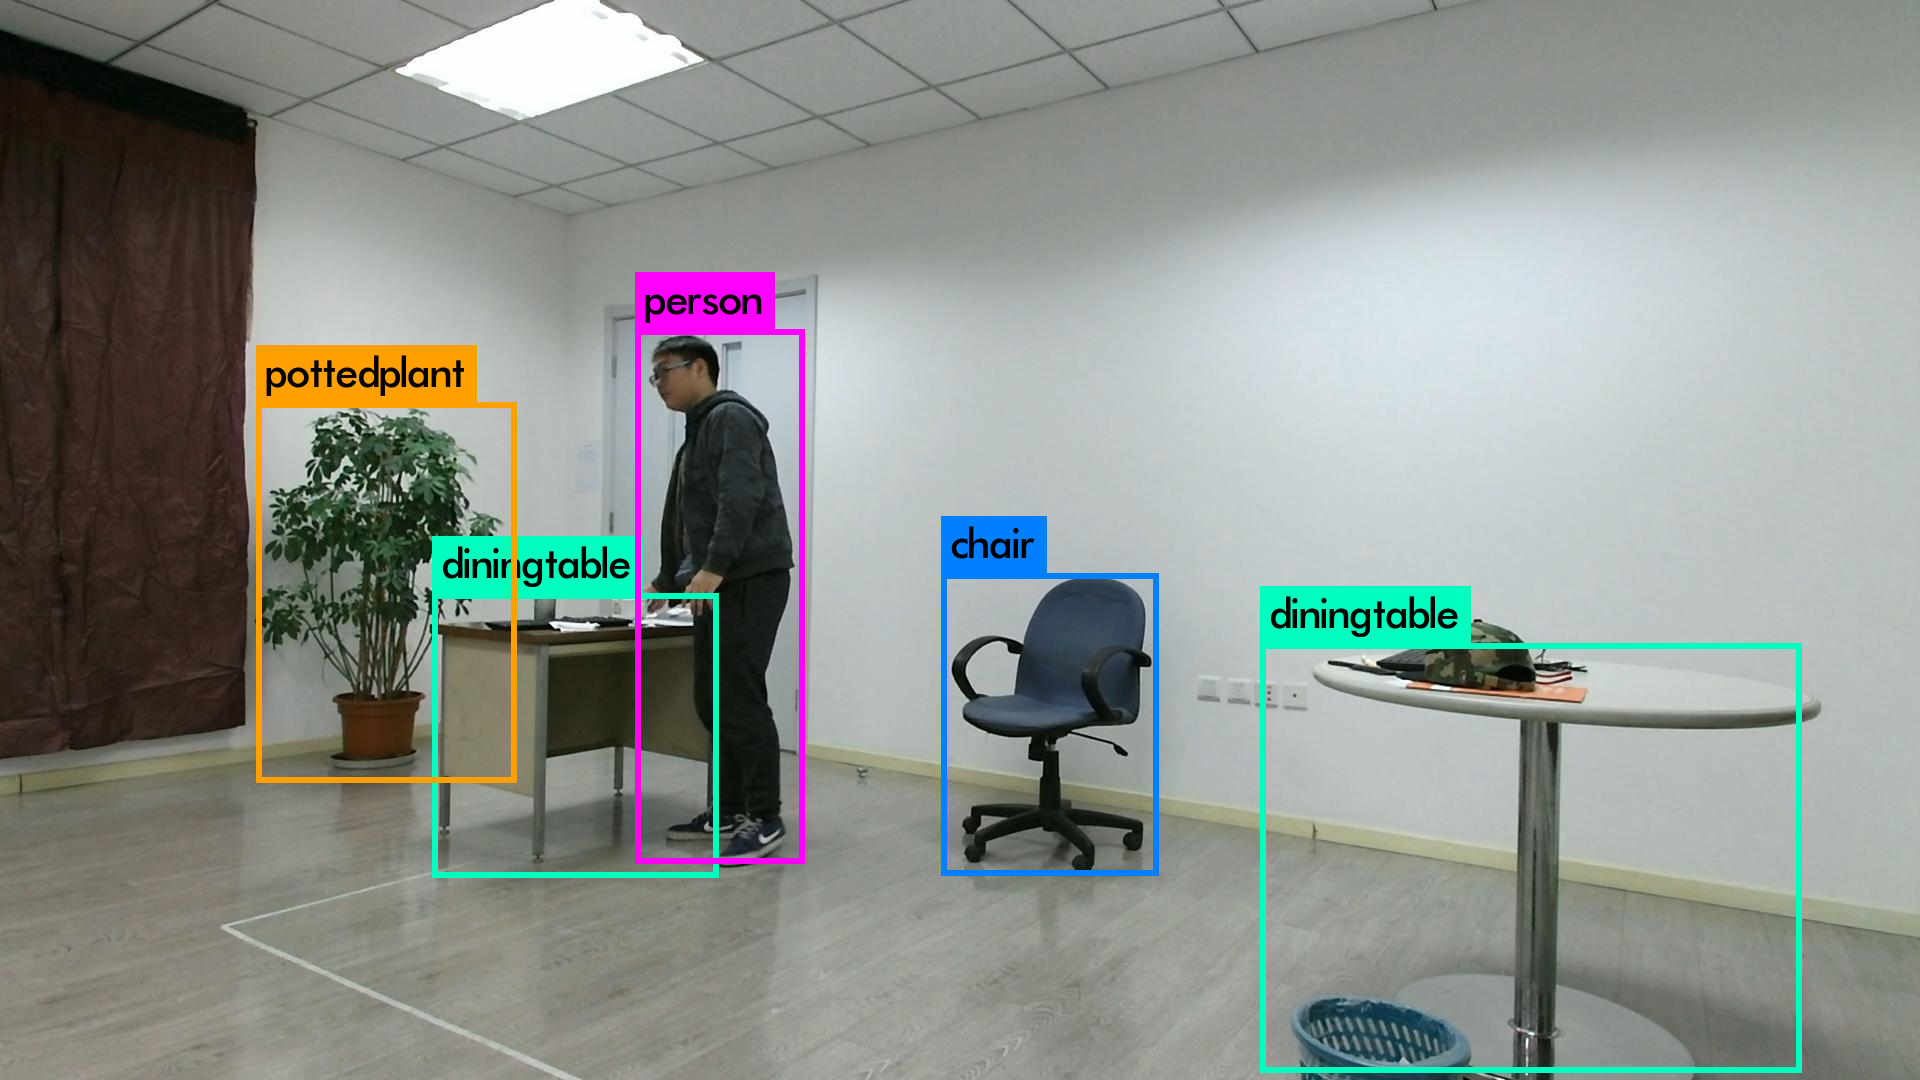
\includegraphics[width=6in,height=4in]{figures/predictions}
	\linebreak
	\captionof{figure}{Detection on PKU-MMD data frame.}
	\label{fig1:PKUMMD-Example}
\end{figure}

\section{Fisher Vector Encoding}
To evaluate the performance of IDT, we used a standard FV approach. A codebook for each descriptor is constructed (trajectory, HOG, HOF, MBH) and a codebook is constructed for the combination of all descriptors. The different number of centers were used which varies from 32 to 256. We fixed it to 64 in our experiments because the performance is very stable compared to other number of centers. 
Note, the FV encoded descriptor dimension for each video is  $1 \times 54528$. To avoid the curse of dimensionality and reduce the computational burden, feature dimensions are further reduced to 400 using PCA. SVM and LibSVM with Linear Kernel are employed for classification.

\section{Experimental Setting}
The IDT code was compiled using the same setting as described in~\cite{HengWang:2011:ARD:2191740.2192078}. We complied this code on 16GB Linux (Ubuntu 16.04) machine with i7-7700k (4.2 GHz). In order to compile the IDT code, Opencv 2.4.11 and ffmpeg-0.11.1 were installed on the machine. The rest of the experiments were performed using MATLAB R2017a. 
%The IDT code is compiled on 16GB Linux machine with i7-7700k (4.2 GHz). In order to compile the IDT code, Opencv 2.4.11 and ffmpeg-0.11.1 were installed on the machine. The rest of the experiments were performed using MATLAB R2017a on 32GB Windows machine with i7-7700k @ 4.2 GHz with 4 cores.










	\chapter{Experimental Results}
\label{resuls}
%\pagenumbering{arabic} 
In this chapter, we will evaluate:
\begin{itemize}
	\item Different IDT descriptors for the single view action recognition
	\item Cross-view action recognition results with/without transfer learning
	\item Cross-view action recognition results with joint dictionary and transfer learning
\end{itemize}
Detailed results and model parameters analysis will be found in the following sections.

\section{Comparison of Different Descriptors}

Different IDT descriptors are compared to check the performance of each individual descriptor (i.e., HOG, HOF, MBH, TRA) and their combination of all descriptors for each view. The results of MBH are the combination of MBHx, and MBHy channel.\ 
The results in Table~\ref{table1} show that IDT descriptor performance is better than other descriptors for the single view recognition, so this motivates us to apply IDT descriptor for later action recognition experiments.
\begin{table}[h]
	\small
	%\large
	\centering
	\caption{Comparison of IDT descriptors on single view classification.} 
	%\resizebox{\textwidth}{!} {%
	\begin{tabular}{@{\extracolsep{12pt}}llcccc}
		\toprule   
		Data & HOF & HOG & MBH & TRA & IDT\\ 
		\hline
		\midrule
		View1  & 94.25\% & 93.10\% & 95.40\% & 81.60\% & 93.10\%\\
		View2  & 96.55\% & 89.65\% & 64.58\% & 77.61\% & 100\%\\
		View3  & 93.10\% & 93.10\% & 94.20\% & 80.06\% & 97.70\%\\
		\bottomrule
		\hline
		\midrule
	\end{tabular}%
	%	}
	\label{table1}
\end{table}

\section{Cross-View Action Recognition without TL}

To conduct ablation study and show the effectiveness of our joint modeling, first, cross-view action recognition is carried out without using any transfer learning method. The model is trained on Fisher Vector encoded video descriptors after applying dimension reduction with PCA. Basically, the model is trained on one view and tested on another view. In the meanwhile, the single view recognition result is also shown to compare the cross-view results. The results are shown in Table~\ref{table3}. We can see that the single view accuracy (on the diagonal) is between 95\% and 100\% while the cross-view accuracy for different cross-view settings are between 40\% and 55\%, which is much more challenging.
\begin{table}[!ht]
	\centering
	\caption{Cross-view action recognition without TL.} 
	%	\resizebox{\textwidth}{!} {%
	\begin{tabular}{@{\extracolsep{40pt}}cccc}
		\toprule   
		{} &   \multicolumn{3}{c}{Training Data}  \\
		\cmidrule{2-4} 
		Testing Data  & View1 & View2 & View3  \\ 
		\hline
		\midrule
		View1  & 96\% & 44.93\% & 45.26\%  \\ 
		View2  & 41.93\% & 100\% & 48.87\%  \\ 
		View3  & 45.55\% & 52.82\% & 98.85\%  \\ 
		\bottomrule
		\hline
		\midrule
	\end{tabular}%
	%	}
	\label{table3}
\end{table}

\section{Cross-View Action Recognition by TL Methods.}

In this section, different transfer learning methods are applied for cross-view settings, and compared with results without using the transfer learning method under the same setting. The evaluation is done using the four state-of-the-art methods, i.e., TCA, TJM, JDA, and BDA, and their details can be found from the methodology section. 

\noindent
\textbf{Parameters Setting}. Note we do not apply PCA for dimension reduction as all transfer learning methods implement dimension reduction by themselves. For all methods $\lambda$ is set to 1, $\gamma$ is set to 0.1 as given in~\cite{6751384}, and number of dimensions are set to 400. The iteration number is set to 5 due to its performance for all methods except TCA since it is not an iterative process. The BDA requires $\mu$ value which is set to 0 as it provided by default in their package and the linear kernel SVM is used for all methods. 

Results for cross-view action recognition using different transfer learning methods are listed in Table~\ref{table2}. From the table, we can see JDA renders higher accuracy in comparison to all other methods, while TJM results are close to JDA results for cross-view action recognition from View2 to View3 and the results for TCA and BDA are between 45\% and 60\%. This indicates that Transfer Learning methods are performing better as compared to the normal approach without knowledge transfer.
\begin{table}[h]
	\centering
	\caption{Cross-view action recognition by TL methods.} 
	%	\resizebox{\textwidth}{!} {%
	\begin{tabular}{@{\extracolsep{40pt}}cccccc}
		\toprule   
		Source & Target & TCA & TJM & JDA & BDA\\ 
		\hline
		\midrule
		View1  & View2 & 47.04\% & 56.22\% & 71.53\% & 53.22\%\\
		View2  & View1 & 59.47\% & 72.81\% & 71.82\% & 59.37\%\\
		View1  & View3 & 62.18\% & 64.58\% & 69.83\% & 42.92\%\\
		View3  & View1 & 47.38\% & 63.09\% & 72.39\% & 45.92\%\\
		View2  & View3 & 52.97\% & 71.67\% & 72\% & 49.43\%\\
     	View3  & View2 & 55\% & 74.96\% & 75.67\% & 57.99\%\\		
		\bottomrule
		\hline
		\midrule
	\end{tabular}%
	%}
	\label{table2}
\end{table}


\section{Cross-View Action Recognition by DL Method}

In this section, cross-view action recognition is carried out on the dictionary learning features. The model is trained on Fisher Vector encoded video descriptors after applying PCA. The model is trained on one view and tested on another view and the single view recognition result is also shown. The results given in Table~\ref{table3:DL} demonstrate that the single view accuracy is between 95\% and 100\% while cross-view accuracies are between 40\% and 55\%.
\begin{table}[!ht]
	\centering
	\caption{Cross-view action recognition by DL.} 
	%	\resizebox{\textwidth}{!} {%
	\begin{tabular}{@{\extracolsep{40pt}}cccc}
		\toprule   
		{} &   \multicolumn{3}{c}{Training Data}  \\
		\cmidrule{2-4} 
		Testing Data  & View1 & View2 & View3  \\ 
		\hline
		\midrule
		View1  & 85.05\% & 42.18\% & 34.13\%  \\ 
		View2  & 42.18\% & 94.25\% & 49.08\%  \\ 
		View3  & 42.03\% & 45.06\% & 91.95\%  \\ 
		\bottomrule
		\hline
		\midrule
	\end{tabular}%
	%	}
	\label{table3:DL}
\end{table}
%Our method approach
\section{Cross-View Action Recognition by JDTL}
% Highlighted Values\
In this section, we will evaluate our proposed joint learning approach for cross-view action recognition where the model is trained on one view and tested on another view. Table~\ref{table4:topnovel} summarizes the highest accuracy achieved by our novel approach using different cross-view settings and different transfer learning methods. From the table, we can see that TCA is performing well, as accuracy is greater than 90\% for all cross-view combinations. The highest accuracy we got using JDA is 92\%, while BDA and TJM accuracy is between 85\% and 95\%. 


\begin{table}[!ht]
	\centering
	\caption{Cross-view action recognition by JDTL.} 
	%	\resizebox{0.9\textwidth}{2cm} {%
	\begin{tabular}{@{\extracolsep{20pt}}cccccc}
		\toprule   
		Training Data & Testing Data &  TCA & JDA & BDA & TJM\\ 
		\hline
		\midrule
		View1&  View2	& 92.8\%  & 92.01\% &	94.51\%	 &91.77\%\\
		View1&	View3	& 94.02\%  &	89.98\%	&	93.38\%	&	83.84\%\\
		View2&	View1	& 91.34\% &	91.50\%	&	92.48\%	&	90.69\%\\
		View2&  View3	& 96.61\% &	92.41\%	&	90.47\%	&	92.89\%\\
		View3&	View1	& 91.83\% &	88.56\%	&	92.32\%	&	88.24\%\\
		View3&	View2	& 90.32\% &	86.94\%	&	88.55\%	&	85.65\%\\
		\bottomrule
		\hline
		\midrule
	\end{tabular}%
	%	}
	\label{table4:topnovel}
\end{table}
%\noindent
Next, we will lead detailed discussions on three different cross-view settings. As our method works in an iterative way to optimize the features, we are allowed to observe the accuracy change in each iteration for different transfer learning methods. The following sections also discuss the confusion matrix where we are allowed for further diagnosis for our cross-view model.

\subsection{Cross-View Action Recognition by JDTL on View1 and View2}

Table~\ref{table5} and Figure~\ref{fig1:View1-View2} show the results of cross-view action recognition by training the model on View1 and testing on View2 using our novel proposed approach. Table~\ref{table8} and Figure~\ref{fig1:View2-View1} show the results of cross-view action recognition by training on View2 and testing on View1. From these cross-view settings, we can see that BDA and JDA (supervised learning mode) performance is increasing in each iteration and BDA also handles class imbalance. TCA performance in the first six iterations is increasing, but after that there is a small decrease in accuracy of each iteration.%\\

\begin{table}[hbt!]
	\centering
	\caption{Cross-view action recognition by JDTL trained on View1 and tested on View2.} 
	%	\resizebox{0.9\textwidth}{3cm} {%
	\begin{tabular}{@{\extracolsep{12pt}}ccccc}
		\toprule 
		Iteration No. &  TCA & JDA & BDA & TJM\\ 
		\hline
		\midrule
		1 &79.83\%	& 69.03\% &	82.41\%	 &85.16\%\\
		2&	92.25\%	&	73.38\%	&	90.32\%	&	91.77\%\\
		3&	90.8\%	&	70.48\%	&	88.38\%	&	85.8\%\\
		4&	89.67\%	&	80.96\%	&	92.58\%	&	79.51\%\\
		5&	93.54\%	&	87.74\%	&	94.03\%	&	75.84\%\\
		6&	92.25\%	&	90.32\%	&	92.51\%	&	78.81\%\\
		7&	90.96\%	&	90.01\%	&	94.51\%	&	81.77\%\\
		8&	87.74\%	&	92.01\%	&	92.1\%	&	84.7\%\\
		9&	88.06\%	&	91.93\%	&	91.61\%	&	82.6\%\\
		10&	86.45\%	&	91.61\%	&	92.1\%	&	87.41\%\\
		\bottomrule
		\hline
		\midrule
	\end{tabular}%
%	}
	\label{table5}
\end{table}
%\noindent
Confusion matrices are illustrated in Figure~\ref{fig:CMV1V2} and~\ref{fig:CMV2V1} to identify which actions cause confusion with other actions.
Each column represents the ground truth, while each row represents the predicted results.
As seen from Figure~\ref{fig:CMV1V2}, our model presents appealing results using different transfer learning methods for most action classes in cross-view action recognition such as \enquote{Brushing Teeth}, \enquote{Check Time} and \enquote{Cheer Up}. The accuracy of JDA and BDA is relatively worse, because for most of the cases, one of the action classes are not recognized properly, e.g., \enquote{Bow}.
\begin{figure}[hbt!]
		\centering
	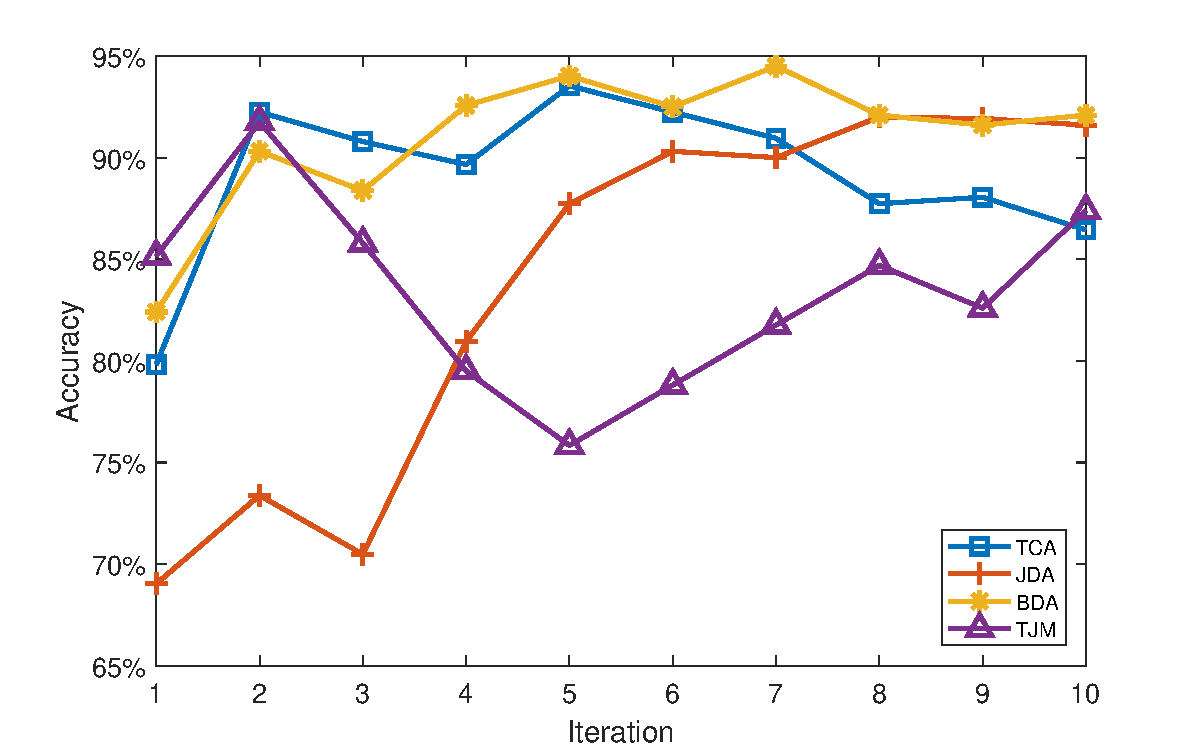
\includegraphics[width=5in,height=3.5in]{figures/plots/View1-View2-2}
	\linebreak
	\caption{Cross-view action recognition by JDTL trained on View1 and tested on View2.}
	\label{fig1:View1-View2}
\end{figure}
%\noindent
Figure~\ref{fig:CMV2V1} shows the confusion matrices when the model is trained on View2 and tested on View1. All classes are properly classified in BDA except \enquote{Brushing Teeth} which is mostly confused with \enquote{Bow} action. The \enquote{Bow} action is creating confusion for other transfer learning methods, such as in TCA, it is confused with \enquote{Cheer Up} action, while in JDA and TJM, it is recognized as \enquote{Brushing Hair}.
%View2-VIew1
\begin{figure}[]
	\centering
	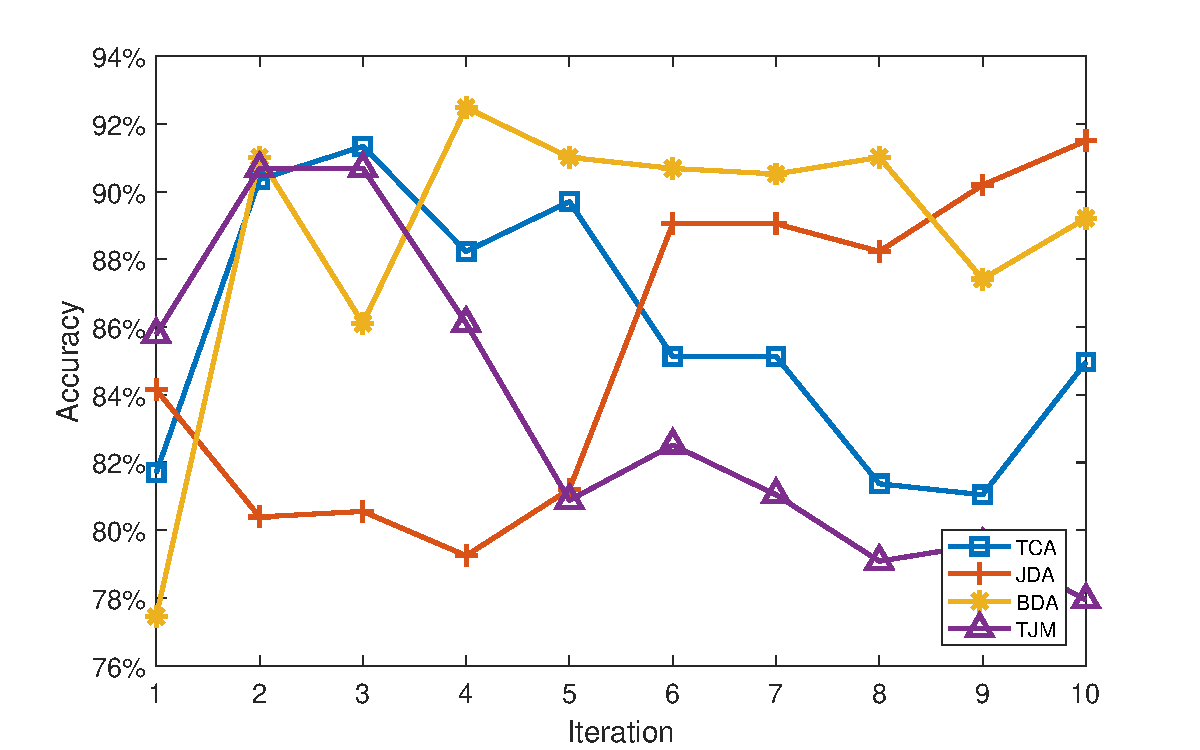
\includegraphics[width=5in,height=3.5in]{figures/plots/View2-View1}
	\linebreak
	\caption{Cross-view action recognition by JDTL trained on View2 and tested on View1.}
	\label{fig1:View2-View1}
\end{figure}

\begin{table}[]
	\centering
	\caption{Cross-view action recognition by JDTL trained on View2 and tested on View1.} 
	%	\resizebox{0.95\textwidth}{3cm} {%
	\begin{tabular}{@{\extracolsep{12pt}}ccccc}
		\toprule   
		Iteration No. &  TCA & JDA & BDA & TJM\\ 
		\hline
		\midrule
		1&	81.70\%&	84.15\%&	77.45\%&	85.78\%\\
		2&	90.36\%&	80.39\%&	91.01\%&	90.69\%\\
		3&	91.34\%&	80.56\%&	86.11\%&	90.69\%\\
		4&	88.24\%&	79.25\%&	92.48\%&	86.11\%\\
		5&	89.71\%&	81.21\%&	91.01\%&	80.88\%\\
		6&	85.13\%&	89.05\%&	90.69\%&	82.52\%\\
		7&	85.13\%&	89.05\%&	90.52\%&	81.05\%\\
		8&	81.37\%&	88.24\%&	91.01\%&	79.08\%\\
		9&	81.05\%&	90.20\%&	87.42\%&	79.58\%\\
		10&	84.97\%&	91.50\%&	89.22\%&	77.94\%\\
		\bottomrule
		\hline
		\midrule
	\end{tabular}%
	%		}
	\label{table8}
\end{table}


\begin{figure}[H]
	\begin{subfigure}{.5\textwidth}
		\centering
		\includegraphics[width=1\linewidth]{"figures/Confusion matrix/BDA/View1View2/V1V2BDA".png}
		\caption{BDA}
		\label{fig:V1V2BDA}
	\end{subfigure}%
	\begin{subfigure}{.5\textwidth}
		\centering
		\includegraphics[width=1\linewidth]{"figures/Confusion matrix/TCA/View1View2/V1V2TCA".png}
		\caption{TCA}
		\label{fig:V1V2TCA}
	\end{subfigure}
	\begin{subfigure}{.5\textwidth}
		\centering
		\includegraphics[width=1\linewidth]{"figures/Confusion matrix/JDA/View1View2/V1V2JDA".png}
		\caption{JDA}
		\label{fig:V1V2JDA}
	\end{subfigure}%
	\begin{subfigure}{.5\textwidth}
		\centering
		\includegraphics[width=1\linewidth]{"figures/Confusion matrix/TJM/View1View2/V1V2TJM".png}
		\caption{TJM}
		\label{fig:V1V2TJM}
	\end{subfigure}
	\caption{Confusion matrix trained on View1 and tested on View2}
	\label{fig:CMV1V2}
\end{figure}



\begin{figure}[H]
	\begin{subfigure}{.5\textwidth}
		\centering
		\includegraphics[width=1\linewidth]{"figures/Confusion matrix/BDA/View2View1/V2V1BDA".png}
		\caption{BDA}
		\label{fig:V2V1BDA}
	\end{subfigure}%
	\begin{subfigure}{.5\textwidth}
		\centering
		\includegraphics[width=1\linewidth]{"figures/Confusion matrix/TCA/View2View1/V2V1TCA".png}
		\caption{TCA}
		\label{fig:V2V1TCA}
	\end{subfigure}
	\begin{subfigure}{.5\textwidth}
		\centering
		\includegraphics[width=1\linewidth]{"figures/Confusion matrix/JDA/View2View1/V2V1JDA".png}
		\caption{JDA}
		\label{fig:V2V1JDA}
	\end{subfigure}%
	\begin{subfigure}{.5\textwidth}
		\centering
		\includegraphics[width=1\linewidth]{"figures/Confusion matrix/TJM/View2View1/V2V1TJM".png}
		\caption{TJM}
		\label{fig:V2V1TJM}
	\end{subfigure}
	\caption{Confusion matrix trained on View2 and tested on View1.}
	\label{fig:CMV2V1}
\end{figure}


\subsection{Cross-View Action Recognition by JDTL on View1 and View3}

Here, we trained the model on View1 and tested on View3 and vice versa. Table~\ref	{table5} and Figure~\ref{fig1:View1-View3} summarize the results for View1 to View3 while Table~\ref{table8} and Figure~\ref{fig1:View3-View1} show the results for View3 to View1. View1 and View3 have mirror videos as those are captured in exact opposite angles. From Figure~\ref{fig1:View1-View3}, we can see that TCA and BDA methods are performing well while JDA and TJM do not have such good results. But in Figure~\ref{fig1:View3-View1}, we can see BDA is performing well as compared to the other methods. The accuracy is increasing for the first five iterations in BDA, and then it is varying with each iteration. In TCA, performance of the first three iteration is increasing, and then it is decreasing with each iteration. The accuracy of JDA and TJM methods does not change too much with each iteration.
\begin{table}[hbt!]
	\centering
	\caption{Cross-view action recognition by JDTL trained on View1 and tested on View3.} 
	%\resizebox{0.7\textwidth}{3cm} {%
		\begin{tabular}{@{\extracolsep{12pt}}ccccc}
			\toprule   
			Iteration No. &  TCA & JDA & BDA & TJM\\ 
			\hline
			\midrule
			1&	86.75\%&	80.29\%&	86.27\%&	70.44\%\\
			2&	90.31\%&	77.38\%&	89.98\%&	67.53\%\\
			3&	91.11\%&	73.02\%&	93.38\%&	67.04\%\\
			4&	92.41\%&	70.60\%&	93.05\%&	69.79\%\\
			5&	94.02\%&	80.45\%&	91.92\%&	72.54\%\\
			6&	91.76\%&	82.07\%&	87.40\%&	73.51\%\\
			7&	93.70\%&	79.97\%&	88.85\%&	78.35\%\\
			8&	92.73\%&	83.52\%&	86.59\%&	77.71\%\\
			9&	92.25\%&	85.62\%&	85.46\%&	83.68\%\\
			10&	93.38\%&	89.98\%&	89.34\%&	83.84\%\\
			\bottomrule
			\hline
			\midrule
		\end{tabular}%
%	}
	\label{table6}
\end{table}

\begin{figure}[hbt!]
	\centering
	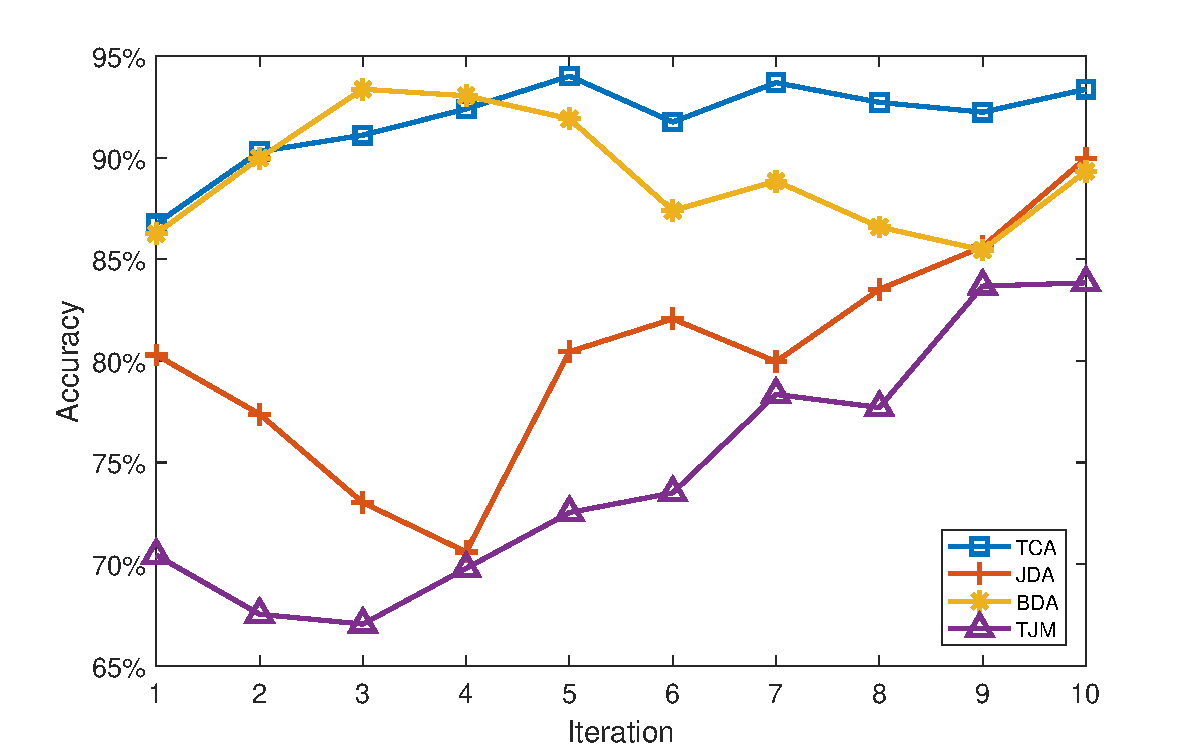
\includegraphics[width=5in,height=3.25in]{figures/plots/View1-View3}
	\linebreak
	\caption{Cross-view action recognition by JDTL trained on View1 and tested on View3.}
	\label{fig1:View1-View3}
\end{figure}


\begin{table}[hbt!]
	\centering
	\caption{Cross-view action recognition by JDTL trained on View3 and tested on View1.} 
	%\resizebox{0.7\textwidth}{3cm} {%
		\begin{tabular}{@{\extracolsep{12pt}}ccccc}
			\toprule
			Iteration No. &  TCA & JDA & BDA & TJM\\ 
			\hline
			\midrule
			1&	70.42\%&	84.31\%&	72.22\%&	79.90\%\\
			2&	87.25\%&	86.93\%&	88.07\%&	84.48\%\\
			3&	91.83\%&	86.93\%&	90.52\%&	86.44\%\\
			4&	87.58\%&	84.31\%&	87.91\%&	86.11\%\\
			5&	85.46\%&	88.56\%&	92.32\%&	85.29\%\\
			6&	85.62\%&	82.35\%&	88.40\%&	85.13\%\\
			7&	84.80\%&	84.31\%&	89.22\%&	85.46\%\\
			8&	84.64\%&	86.60\%&	88.07\%&	86.76\%\\
			9&	84.15\%&	85.95\%&	90.52\%&	88.24\%\\
			10&	83.33\%&	85.29\%&	90.36\%&	86.44\%\\
			\bottomrule
			\hline
			\midrule
		\end{tabular}%
%	}
	\label{table9}
\end{table}


\begin{figure}[hbt!]
	\centering
	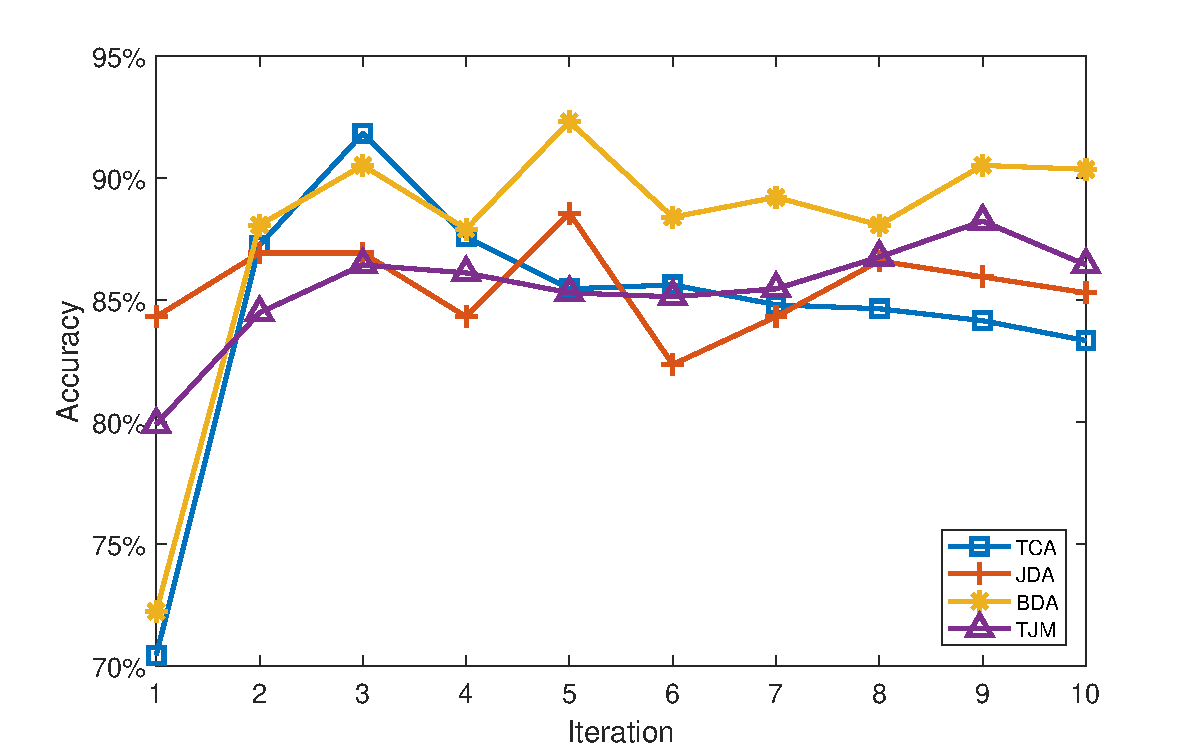
\includegraphics[width=5in,height=3.5in]{figures/plots/View3-View1}
	\linebreak
	\caption{Cross-view action recognition by JDTL trained on View3 and tested on View1.}
	\label{fig1:View3-View1}
\end{figure}

Confusion matrices for these cross-view combinations are given in Figure~\ref{fig:CMV1V3} and Figure~\ref{fig:CMV3V1} for View1 to View3 and View3 to View1, respectively. Figure~\ref{fig:CMV1V3} shows that in BDA and TJM \enquote{Brushing Teeth} is misclassified as \enquote{Check Time} or \enquote{Cheer Up}, while in TCA \enquote{Brushing Hair} and \enquote{Check Time} are mostly confused with each other. From Figure~\ref{fig:CMV3V1}, it can be seen that \enquote{Bow} action is misclassified with all other actions in BDA, JDA and TJM methods, while in JDA and BDA methods \enquote{Cheer Up} action is recognized correctly. In TCA \enquote{Brushing Hair} is misclassified with \enquote{Check Time} and \enquote{Cheer Up} actions.
%% View1 -View 3 table and plot

%% View3- VIew1




\begin{figure}[]
	\begin{subfigure}{.5\textwidth}
		\centering
		\includegraphics[width=1\linewidth]{"figures/Confusion matrix/BDA/View1View3/V1V3BDA".png}
		\caption{BDA}
		\label{fig:V1V3BDA}
	\end{subfigure}%
	\begin{subfigure}{.5\textwidth}
		\centering
		\includegraphics[width=1\linewidth]{"figures/Confusion matrix/TCA/View1View3/V1V3TCA".png}
		\caption{TCA}
		\label{fig:V1V3TCA}
	\end{subfigure}
	\begin{subfigure}{.5\textwidth}
		\centering
		\includegraphics[width=1\linewidth]{"figures/Confusion matrix/JDA/View1View3/V1V3JDA".png}
		\caption{JDA}
		\label{fig:V1V3JDA}
	\end{subfigure}%
	\begin{subfigure}{.5\textwidth}
		\centering
		\includegraphics[width=1\linewidth]{"figures/Confusion matrix/TJM/View1View3/V1V3TJM".png}
		\caption{TJM}
		\label{fig:V1V3TJM}
	\end{subfigure}
	\caption{Confusion matrix trained on View1 and tested on View3}
	\label{fig:CMV1V3}
\end{figure}

\begin{figure}[]
	\begin{subfigure}{.5\textwidth}
		\centering
		\includegraphics[width=1\linewidth]{"figures/Confusion matrix/BDA/View3View1/V3V1BDA".png}
		\caption{BDA}
		\label{fig:V3V1BDA}
	\end{subfigure}%
	\begin{subfigure}{.5\textwidth}
		\centering
		\includegraphics[width=1\linewidth]{"figures/Confusion matrix/TCA/View3View1/V3V1TCA".png}
		\caption{TCA}
		\label{fig:V3V1TCA}
	\end{subfigure}
	\begin{subfigure}{.5\textwidth}
		\centering
		\includegraphics[width=1\linewidth]{"figures/Confusion matrix/JDA/View3View1/V3V1JDA".png}
		\caption{JDA}
		\label{fig:V3V1JDA}
	\end{subfigure}%
	\begin{subfigure}{.5\textwidth}
		\centering
		\includegraphics[width=1\linewidth]{"figures/Confusion matrix/TJM/View3View1/V3V1TJM".png}
		\caption{TJM}
		\label{fig:V3V1TJM}
	\end{subfigure}
	\caption{Confusion matrix trained on View3 and tested on View1.}
	\label{fig:CMV3V1}
\end{figure}

%% View2 -View2 table and plot
%% View2 -View 3 table and plot
\subsection{Cross-View Action Recognition by JDTL on View2 and View3}
Table~\ref{table7} and Figure~\ref{fig1:View2-View3} show the results for cross-view action recognition when the model is trained on View2 and tested on View3 and Table~\ref{table10} and Figure~\ref{fig1:View3-View2} show the results when the model is trained on View3 and tested on View2. We can see in Figure~\ref{fig1:View2-View3}, TCA accuracy is increasing until the seventh iteration and then it is decreasing. In BDA, accuracy increases until sixth iteration and in TJM it increases until fourth iteration. Then performance decreases in both methods. In JDA, accuracy increases until fifth iteration and then it is changing with different iterations.

The Figure~\ref{fig:CMV2V3} shows which action classes are creating confusion when the model is trained on View2 and tested on View3. From the confusion matrices, we can see that \enquote{Bow} action is creating the confusion in BDA, JDA, and TJM transfer learning methods. While in TCA \enquote{Brushing Teeth} is recognized as the \enquote{Cheer Up} or \enquote{Bow} actions.
\begin{figure}[hbt!]
	\centering
	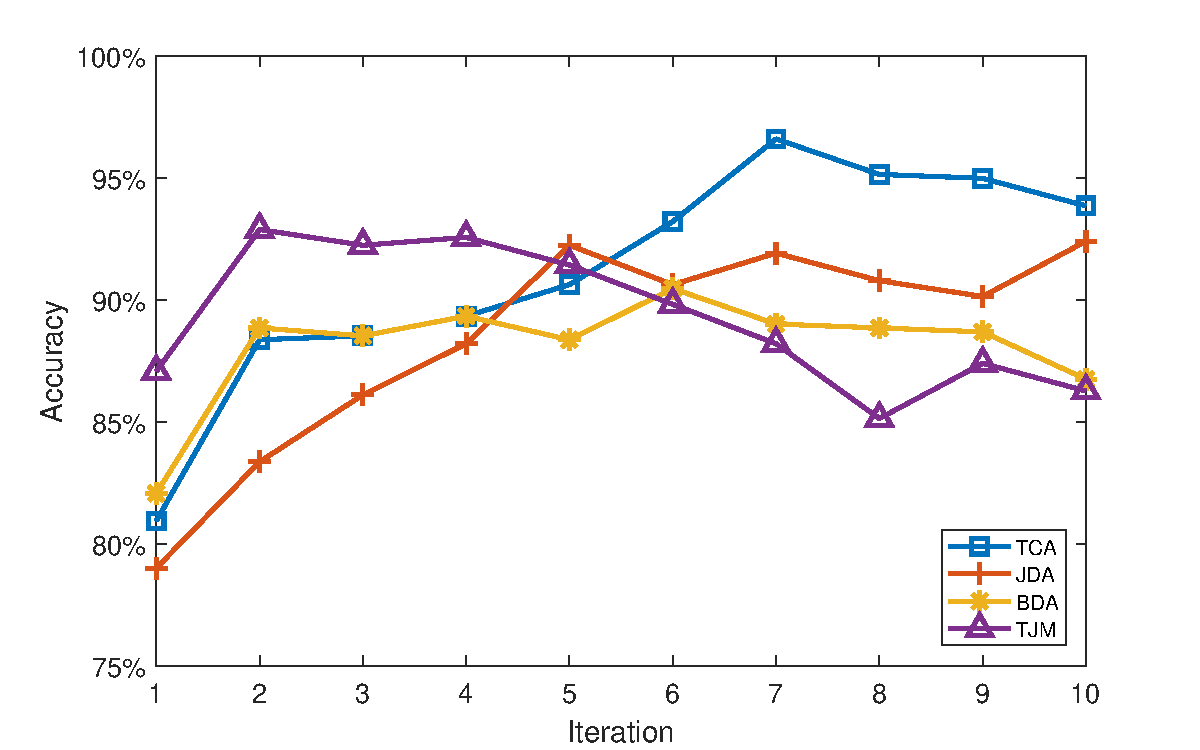
\includegraphics[width=5in,height=3.25in]{figures/plots/View2-View3}
	\linebreak
	\caption{Cross-view action recognition by JDTL trained on View2 and tested on View3.}
	\label{fig1:View2-View3}
\end{figure}

\begin{table}[]
	\centering
	\caption{Cross-view action recognition by JDTL trained on View2 and tested on View3.} 
	%\resizebox{0.7\textwidth}{!} {%
	\begin{tabular}{@{\extracolsep{12pt}}ccccc}
		\toprule   
		Iteration No. &  TCA & JDA & BDA & TJM\\ 
		\hline
		\midrule
		1&	80.94\%&	79.00\%&	82.07\%&	87.08\%\\
		2&	88.37\%&	83.36\%&	88.85\%&	92.89\%\\
		3&	88.53\%&	86.11\%&	88.53\%&	92.25\%\\
		4&	89.34\%&	88.21\%&	89.34\%&	92.57\%\\
		5&	90.63\%&	92.25\%&	88.37\%&	91.44\%\\
		6&	93.21\%&	90.63\%&	90.47\%&	89.82\%\\
		7&	96.61\%&	91.92\%&	89.01\%&	88.21\%\\
		8&	95.15\%&	90.79\%&	88.85\%&	85.14\%\\
		9&	94.99\%&	90.15\%&	88.69\%&	87.40\%\\
		10&	93.86\%&	92.41\%&	86.75\%&	86.27\%\\
		\bottomrule
		\hline
		\midrule
	\end{tabular}%
	%	}
	\label{table7}
\end{table}

%% View3- View2
\begin{figure}[]
	\centering
	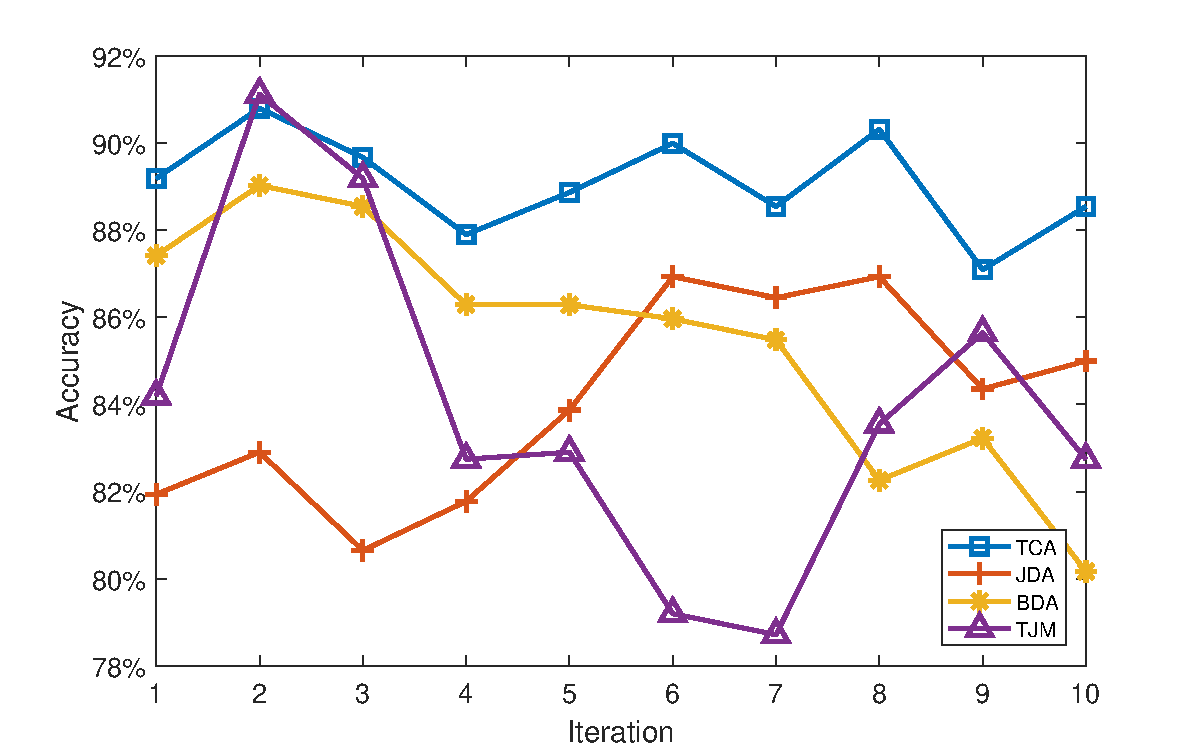
\includegraphics[width=5in,height=3.25in]{figures/plots/View3-View2}
	\linebreak
	\caption{Cross-view action recognition by JDTL trained on View3 and tested on View2.}
	\label{fig1:View3-View2}
\end{figure}

\begin{table}[hbt!]
	
	\centering
	\caption{Cross-view action recognition by JDTL trained on View3 and tested on View2.} 
	%	\resizebox{0.75\textwidth}{!} {%
	\begin{tabular}{@{\extracolsep{12pt}}ccccc}
		\toprule   
		Iteration No. &  TCA & JDA & BDA & TJM\\ 
		\hline
		\midrule
		1&	89.19\%&	81.94\%&	87.42\%&	84.19\%\\
		2&	90.81\%&	82.90\%&	89.03\%&	91.13\%\\
		3&	89.68\%&	80.65\%&	88.55\%&	89.19\%\\
		4&	87.90\%&	81.77\%&	86.29\%&	82.74\%\\
		5&	88.87\%&	83.87\%&	86.29\%&	82.90\%\\
		6&	90.00\%&	86.94\%&	85.97\%&	79.19\%\\
		7&	88.55\%&	86.45\%&	85.48\%&	78.71\%\\
		8&	90.32\%&	86.94\%&	82.26\%&	83.55\%\\
		9&	87.10\%&	84.35\%&	83.23\%&	85.65\%\\
		10&	88.55\%&	85.00\%&	80.16\%&	82.74\%\\
		\bottomrule
		\hline
		\midrule
	\end{tabular}%
	%	}
	\label{table10}
\end{table}

From Figure~\ref{fig1:View3-View2}, we can see that the highest accuracy for TCA, JDA, and TJM is achieved in the second iteration, while in JDA it is achieved in sixth and eighth iteration. As we can see in Figure~\ref{fig1:View3-View2} that JDA accuracy seems to be increasing after third iteration while BDA accuracy is decreasing after second iteration. The accuracy of TCA is stabilized over the iteration while TJM is very unstable. The confusion matrix for this cross-view combination is shown in Figure~\ref{fig:CMV3V2}. \enquote{Bow} and \enquote{Cheer Up} actions are mostly misclassified with different actions in all transfer learning methods. In TCA and BDA \enquote{Cheer Up} and \enquote{Check Time} are misclassified with each other.

\begin{figure}[hbt!]
	\begin{subfigure}{.5\textwidth}
		\centering
		\includegraphics[width=1\linewidth]{"figures/Confusion matrix/BDA/View2View3/V2V3BDA".png}
		\caption{BDA}
		\label{fig:V2V3BDA}
	\end{subfigure}%
	\begin{subfigure}{.5\textwidth}
		\centering
		\includegraphics[width=1\linewidth]{"figures/Confusion matrix/TCA/View2View3/V2V3TCA".png}
		\caption{TCA}
		\label{fig:V2V3TCA}
	\end{subfigure}
	\begin{subfigure}{.5\textwidth}
		\centering
		\includegraphics[width=1\linewidth]{"figures/Confusion matrix/JDA/View2View3/V2V3JDA".png}
		\caption{JDA}
		\label{fig:V2V3JDA}
	\end{subfigure}%
	\begin{subfigure}{.5\textwidth}
		\centering
		\includegraphics[width=1\linewidth]{"figures/Confusion matrix/TJM/View2View3/V2V3TJM".png}
		\caption{TJM}
		\label{fig:V2V3TJM}
	\end{subfigure}
	\caption{Confusion matrix trained on View2 and tested on View3.}
	\label{fig:CMV2V3}
\end{figure}



\begin{figure}[hbt!]
	\begin{subfigure}{.5\textwidth}
		\centering
		\includegraphics[width=1\linewidth]{"figures/Confusion matrix/BDA/View3View2/V3V2BDA".png}
		\caption{BDA}
		\label{fig:V3V2BDA}
	\end{subfigure}%
	\begin{subfigure}{.5\textwidth}
		\centering
		\includegraphics[width=1\linewidth]{"figures/Confusion matrix/TCA/View3View2/V3V2TCA".png}
		\caption{TCA}
		\label{fig:V3V2TCA}
	\end{subfigure}
	\begin{subfigure}{.5\textwidth}
		\centering
		\includegraphics[width=1\linewidth]{"figures/Confusion matrix/JDA/View3View2/V3V2JDA".png}
		\caption{JDA}
		\label{fig:V3V2JDA}
	\end{subfigure}%
	\begin{subfigure}{.5\textwidth}
		\centering
		\includegraphics[width=1\linewidth]{"figures/Confusion matrix/TJM/View3View2/V3V2TJM".png}
		\caption{TJM}
		\label{fig:V3V2TJM}
	\end{subfigure}
	\caption{Confusion matrix trained on View3 and tested on View2.}
	\label{fig:CMV3V2}
\end{figure}
%\noindent 


\section{Discussion}
From the experimental results, it can be concluded that we obtained significant results from different cross-view settings by training the model on one view and recognizing the same action from different views using our joint dictionary and transfer learning method (JDTL). The effectiveness of our proposed approach has been demonstrated by comparing our models with those trained with, or without transfer learning and dictionary learning methods.

As we have discussed earlier that our method works in an iterative manner, the accuracy of most of the transfer learning methods is increasing until fifth iteration. After that, the performance becomes different, which may be caused by the confusion between two actions. For example, from the confusion matrices, we can learn that mostly \enquote{Bow} action is confused with \enquote{Brushing Hair} action.

The JDTL method is efficient as compared to other cross-view or multi-view action recognition methods because in other methods common feature representation is extracted by constructing a connection or mapping between both views. To that end, videos need to be aligned well based on the frame-to-frame, video-to-video, or codebook-to-codebook criteria. In our method, however, we did not construct any mapping, as dictionary learning is used to extract discriminative features and transfer learning is used to project those discriminative features into common subspace, which provides better time and memory efficacy.

In this study, we evaluated our method on the action classes with only a single person performing some actions in a closed and fixed environment. It will become more complex but attractive in recognizing actions of an individual person when multiple people exist and act differently. This will reflect most real-world scenarios for action recognition. Also, in our study, we considered five action classes for the evaluations, while we may further explore other classes to testify the robustness of our model, and its real-world values.



	\chapter{Conclusions}
\label{conclusion}
In this study, we proposed a new joint learning model to address problem of cross-view action recognition where we trained the model in one view and tested the model in a different view. For this purpose, we developed a joint dictionary and transfer learning framework. The dictionary generated the view-independent discriminative features while the transfer learning projected those discriminative features into a common subspace. Specifically, Improve Dense Trajectory (IDT) visual descriptor is applied for robust action feature extraction. State-of-the-arts transfer learning methods were applied and integrated in our model for comparison. Extended evaluations were done on PKU-MMD multi-view dataset, and our proposed approach showed significant results compared to existing methods.

For the future work, the short-term plan is to extend this work by considering recent deep learning features such as two-stream deep model. It learns the semantic representation from raw data and considers both spatial and temporal information. In addition to this, our proposed approach is only evaluated on five action classes, but we are planning to add more action classes which include interactions between two individuals.
 
In a long-term plan for the improvement and extension of proposed approach, we may consider zero-shot learning and action prediction problem in multi-view setting. In zero-shot learning, a model is constructed on the labeled training set of seen classes to discover the semantic relationship between seen and newly available unseen classes in test data. While the motive for multi-view action prediction problem is to recognize the action (future action) from incomplete action execution where multi-view information can be utilized to avoid the scene loss and recover the blocked and cluttered views. In addition, we will consider improving our approach by recognizing actions of multiple people in a single video.

%\pagenumbering{arabic} 



%%  set the format required for the citations/references
%%  \bibliographystyle{unsrt} is preferred for UMassD theses & dissertations.
\bibliographystyle{ieeetr}
%\bibliography{bibfile}

%%  The document text can be typed directly into this file or make use of
%%  the LaTeX \input{filename} command to read the contents of the file
%%  filename.tex.
%%  The later method is a good way to logically organize the material.

%%  INSERT THESIS BODY HERE

%%  if using the LaTeX \input command 
%\input{introduction}


%%  Everything after this is an appendix

%%
%%  If there is more that ONE appendix
%%
%%\appendix

%%\chapter{Additional Material
%%\label{sample-appendix}}

%%\section{Introduction}
%%\label{sample-appendix:introduction-section}

%%This is a sample appendix. By adding the command $\backslash$appendix to the
%%\LaTeX\ file before this file is included, the Table of Contents will
%%reflect the appendical nature now attained. 

%%\section{Appendictical Numbering}
%%\label{sample-appendix:numbering-section}

%%Appendices are labeled alphabetically rather than numerically as with chapters.
%%Each is identified separately as ``Appendix A'', ``Appendix B'', and so forth. 

%%\section{Getting the labels right \ldots}

%Sections in the first appendix will be labeled A.1, A.2 etc.  Similarly,
%subsections, equations, figures and tables will have a leading A.   This will
%be reflected in the Table of Contents, List of Figures and List of Tables in
%the prologue pages.



%\chapter{The Second Appendix}

%This is labeled Appendix B.

%\section{A Section} 

%Sections within this are labeled B.1

%\section{A Nother Section} 

%Additional sections are labeled B.2 \ldots


%%%
%%%  If there is ONE appendix use the \singleappendix command
%%%
%\singleappendix
%\chapter{The Only Appendix}
%
%If there is only one appendix, it is called ``Appendix'' (not ``Appendix
%A'').  
%
%To achieve this, use the command, {\tt $\backslash$singleappendix}
%
%\section{Appendictical Numbering}
%\label{sample-appendix:numbering-section}
%
%The command, {\tt $\backslash$singleappendix} prints the appendix title without
%the trailing A.
%
%\section{Getting the labels right \ldots}
%
%The {\tt $\backslash$singleappendix} command also ensures that the section and
%subsection numbers don't include a leading A. and  that the the Table of
%Contents, List of Figures and List of Tables entries for section, subsection,
%equations, figures and tables don't have a leading period. 
%


%%
%%  End of any appendices
%%  =========================================================================


%%  At the end of the document are the references. These are single-spaced
%%  rather than double-spaced like the rest of the thesis text.

\begin{singlespace}
   \bibliography{bibfile}
\end{singlespace}


\end{document}
%% ===========
%%    FINI
%% ===========
